\chapter{Materiais e Métodos}
\label{chap:materiais_metodos}
O metodologia empregada nos trabalhos de conclusão de curso do Centro Universitário SENAI CIMATEC é executado com base na metodologia TheoPrax que foi desenvolvida pelo instituto Fraunhofer de Tecnologia Química, situado na Alemanha. A sistemática TheoPrax tem como principal objetivo incrementar a motivação da aprendizagem através do desenvolvimento de projetos reais voltados para empresas, proporcionando a integração entre o conhecimento técnico e sua aplicação prática. Para isto, esta estrutura envolve a identificação de uma situação problema ou de uma melhoria no processo ou no produto da empresa, seu estudo e, por fim, a definição de uma proposta técnica-financeira para implementação da solução.

\section{Metodologia}
\label{sec:metodologia}
A utilização da metodologia TheoPrax se restringe apenas ao gerenciamento macro do projeto e não define como a solução proposta deve ser desenvolvida. Sendo assim, o desenvolvimento do projeto, proposto no tópico \ref{sec:objetivo_geral}, foi realizado utilizando o procedimento ilustrado na figura \ref{fig:metodologia_diagrama} que foi adaptado da metodologia empregada no \gls*{bir} para desenvolvimento de projetos de robótica.

\begin{figure}[H]
	\centering
	\caption{Metodologia empregada no desenlvolvimento do projeto solução.}
	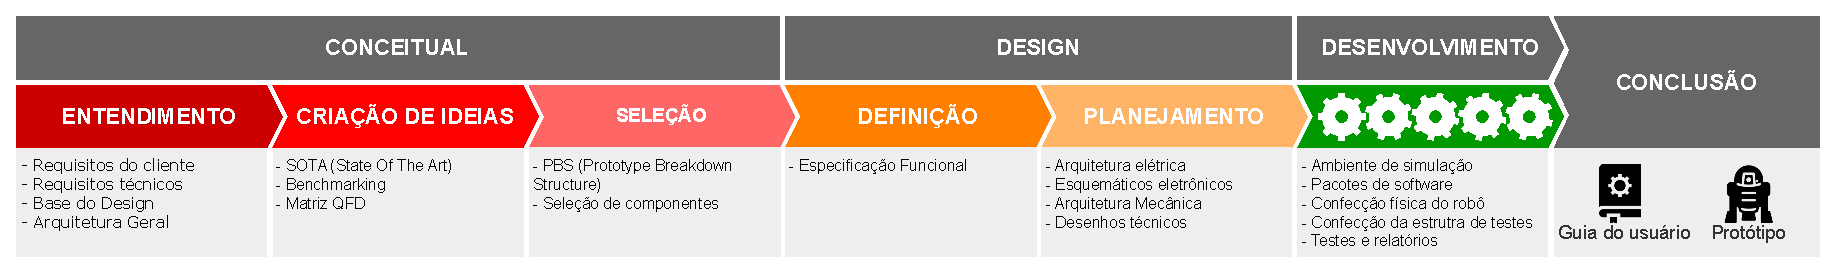
\includegraphics[width=1\textwidth]
	{Figures/metodologia_diagrama}
	\label{fig:metodologia_diagrama}
	\source{Própria Autoria}
\end{figure}	

Conforme Figura \ref{fig:metodologia_diagrama}, a metodologia utilizada neste projeto possui 4 etapas: Conceitual, Design, Desenvolvimento e Conclusão. Por conseguinte, cada etapa possui entradas e saídas, que vão se complementando ao longo do desenvolvimento do projeto, as quais serão explicadas nos tópicos seguintes.

\subsection{Conceitual}
\label{subsec:metodologia_conceitual}

A primeira etapa, designada como \textbf{Conceitual}, embora não explicitada no diagrama, possui como entradas as informações provenientes do cliente. Essas informações, tais como o problema proposto e os seus requisitos são utilizadas para o entendimento do projeto, servindo como ponto de partida para formulação da proposta de solução. Diante dessas informações, é possível definir os requisitos técnicos com base nos desejos do cliente (requisitos do cliente); a base do design, que consiste na definição do escopo e o que será necessário para desenvolver o projeto: meios, padrões e os principais componentes (hardware e software); e a arquiterura geral, que fornece uma visão macro de como será a interação entre o hardware e o software do robô. 

Após o entendimento do projeto, passa-se para a criação de ideias. Nesta subetapa, algumas pesquisas são realizadas para ajudar no processo de criatividade e evitar a reimplementação do que já existe no mercado. Assim, utiliza-se o \gls*{sota}, documento que aponta as principais pesquisas  e estudos sobre o tema do projeto, referenciando pesquisas acadêmicas já realizadas; e o \textit{Benchmarking}, que é uma relação oriunda do mercado na qual aponta os competidores para o sistema projetado, incluindo para cada competidor critérios de avaliações importantes para o projeto. Finalizando a subetapa de criação de ideias, tem-se a Matriz \gls*{qfd}, em que os requisitos do cliente são confrontados com os requisitos técnicos, fornecendo à equipe de desenvolvimento do projeto os principais pontos que deverão receber maior atenção durante a elaboração do projeto. 

Por fim, após o entendimento do projeto e a formulação da ideia, parte-se para a etapa de seleção dos principais componentes do  sistema, em que primeiro elabora-se o \gls*{pbs}, uma representação do projeto com uma visão de subsistemas, apresentado através de um fluxo estruturado.

\subsection{Design}
\label{subsec:metodologia_design}
Com o conceito pré-estabelecido do sistema que será desenvolvido, parte-se para a etapa de \textbf{Design}. Nesta fase, define-se o sistema de maneira mais clara, tendo a especificação funcional como principal elemento. Este documento compreende a explicação  detalhada de cada funcionalidade do robô, contendo a definição, o objetivo, as premissas e as suas entradas e saídas. Devido ao nível de detalhes da especificação funcional, revisões em documentos anteriores, principalmente a arquitetura geral, são realizadas durante esta fase. 

No final da etapa de Design, começa-se o planejamento para o desenvolvimento técnico do projeto. Durante o planejamento é elaborado a arquitetura elétrica do robô (uma visão mais detalhada da arquitetura geral), descrevendo as formas de conexão e os protocolos de comunicação entre os elementos que compõem o sistema; os equemáticos eletrônicos, os quais são utilizados para confecção das \glspl*{pci} que comporão o sistema; a arquitetura mecânica, apresentando os elementos mecânicos do robô; e por fim, os desenhos técnicos mecânicos, utilizados posteriormente para fabricação das peças do protótipo. 

Em conclusão, esta fase é de extrema importância, pois possibilita a geração de documentos que podem ser utilizados para a replicação do projeto. Além do mais, permite mais fluidez no desenvolvimento técnico do robô.

\subsection{Desenvolvimento}
\label{subsec:metodologia_desenvolvimento}

Após a finalização do planejamento, começa-se a etapa de \textbf{Desenvolvimento} do projeto, em que o conceito e as ideias provenientes das etapas anteriores tornam-se concretas. Nesta fase são desenvolvidos e documentados os pacotes de software, os quais englobam tanto a unidade de controle do robô quanto os \textit{drivers} dos sensores, atuadores e elementos de interação com usuário. Muito dos pacotes aqui desenvolvidos, usam a especificação funcional como guia. 

Para auxiliar no processso de desenvolvimento, um ambiente de simulação torna-se elemento vital. O ambiente de simulação permite que ideias sejam propostas e testadas sem a necessidade do uso da plataforma física, acelerando o processo de desenvolvimento num âmbito em que se possui diversas pessoas trabalhando no mesmo sistema. Não menos importante, os simuladores evitam que danos sejam causados ao robô em caso de má implementação de algum algoritmo. 

Entretanto, os ambientes de simulação não refletem completamente os aspectos físicos do mundo real. Diante disso, na fase de desenvolvimento torna-se necessário também a confecção de um ambiente real para testes. Com essa estrutura, também chamada de \textit{Mockup}, pode-se realizar testes para validar o que foi desenvolvido e produzir relatórios que podem ser entregues ao cliente  como forma de acompanhamento do desenvolvimento técnico do projeto.

\subsection{Conclusão}
\label{metodologia_conclusao}
O projeto é finalizado na etapa de \textbf{Conclusão}, em que a solução proposta é entregue ao cliente. Nesta entrega é realizado a demonstração do funcionamento do robô, utilizando um ambiente real. Também é cedido além da documentação elaborada ao longo do desenvolvimento do projeto, um documento em formato de Guia do Usuário contendo as instruções para manipulação e replicação do protótipo desenvolvido.

%--------- NEW SECTION ----------------------

\section{Requisitos do projeto}
\label{sec:requisitos_do_projeto}
Como mencionado no início deste capítulo, uma das etapas da metodologia TheoPrax envolve a identificação de uma situação problema. No projeto em questão, foi solicitado ao cliente os requisitos que o Doogie Mouse deveria cumprir. Entretanto, tais requisitos refletem a vontade do cliente de forma não técnica. Assim, a partir dos requisitos do cliente, foram levantados por parte da equipe de desenvolvimento os requisitos técnicos, os quais fornecem objetivos específicos que o projeto deve atingir. Por consequência, o cumprimento dos requisitos técnicos decorre na aprovação dos requisitos do cliente. Abaixo estão listados os requisitos do cliente e técnicos do Doogie Mouse de forma hierárquica, isto é, para cada requisito do cliente estão listados seus respectivos requisitos técnicos associado.

\begin{enumerate}
	\item Documentação de fácil acesso e entendimento:
	\begin{enumerate}
		\item Disponibilização de todo código desenvolvido no GitHub;
		
		\item Disponibilização guia do usuário como Wiki no GitHub;
		
		\item Disponibilização em um repositório no GitHub esquemáticos eletrônicos, desenhos técnicos mecânicos e seus respectivos arquivos para possível edição.
	\end{enumerate}
	
	\item Uso de um sistema microprocessado comercial:
	\begin{enumerate}
		\item Utilização de uma Raspberry Pi como sistema microprocessado;
	\end{enumerate}
	
	\item Interface intuitiva:
	\begin{enumerate}
		\item Permissão ao usuário acesso remoto do terminal do sistema operacional do robô;
		
		\item Visualização do mapa do Labirinto no RViz;
		
		\item Disponibilização de botões e display para interação com usuário na ausência de acesso remoto.
		
	\end{enumerate}
	
	\item Tutoriais na internet para entendimento do funcionamento do robô:
	\begin{enumerate}
		\item Desenvolvimento de tutorial na \gls*{ros} Wiki com os primeiros passos com robô, explicando ao usuário comandos básicos de locomoção;
		
		\item Desenvolvimento de tutorial na \gls*{ros} Wiki explicando ao usuário como implementar no robô seu próprio algoritmo de resolução de labirinto.
	\end{enumerate}
	
	\item Autonomia suficiente para utilização em ao menos duas aulas consecutivas:
	\begin{enumerate}
		\item Bateria recarregável;
		
		\item Autonomia superior a 1h40min.
	\end{enumerate}
	
	\item Uso de componentes de fácil manipulação e com facilidade de aquisição:
	\begin{enumerate}
		\item Uso de conectores polarizados;
		
		\item Utilização de padrão de cores para cabos de conexão;
		
		\item Especificação de componentes disponíveis no mercado nacional;
		
		\item Desenvolvimento de shield de interface entre a plataforma de processamento e os sensores e atuadores.
	\end{enumerate}
	
	\item Estrutura física compatível com as regras estabelecidas em competições do \gls*{ieee}:
	\begin{enumerate}
		\item Dimensões do robô devem ser menores que 15 x 15 x 10 cm.
	\end{enumerate}
\end{enumerate}

Por fim, para a proporcionar a equipe de desenvolvimento um guia em relação a aplicação dos esforços para que os requisitos do cliente e técnico fossem atingidos, foi realizado uma confrontação de tais requisitos. Esta análise foi derivada de uma ferramenta comumente utilizada em desenvolvimento de produto, denominada matriz \acrshort*{qfd}. A confrontação dos requisitos do projeto proposto pode ser visualizada no Apêndice \ref{apend:matriz_QFD}. Observa-se na linha 5 da matriz que o requisito técnico "Permissão ao usuário de acesso remoto do terminal do sistema operacional do robô" possui apenas uma relação forte com o requisito do cliente "Interface intuitiva". Por outro lado, "Dimensões do robô devem ser menores que 15 x 15 x 10 cm", na linha 16, possui 2 relações fracas, uma média e uma forte com diferentes requisitos do cliente. Portanto, essas associações funcionam como direcionadores de esforços e prioridades das tarefas desenvolvidas ao longo do projeto.

%--------- NEW SECTION ----------------------
\section{Descrição do sistema}
\label{sec:descricao_do_sistema}
O Doogie é um robô autônomo capaz de mapear um labirinto e descobrir qual o menor caminho do seu ponto de partida até um ponto de chegada. Sua arquitetura, ilustrada na Figura \ref{fig:arquitetura_geral}, pode ser dividida em três partes: interação com o usuário, controle do sistema e interface de hardware.
Para a interação com o usuário, o robô possuirá um Buzzer e dois \textit{Push Buttons}. Além disso, há a possibilidade de acessar o sistema do robô via \gls*{ssh}, por intermédio da conexão WiFi. A interface de hardware é composta por motores de corrente contínua, responsáveis pela movimentação, trabalhando em conjunto com uma ponte H e Encoders; sensores infravermelhos, dispostos na frente e dos lados, a fim de identificar paredes; e uma \gls*{imu}, responsável por fornecer a aceleração linear e a velocidade angular da plataforma móvel para complementar os dados de Odometria. O controle do sistema é embarcado dentro de uma Raspberry Pi Zero que utiliza o \textit{framework} \gls*{ros} para gerenciar os diversos subsistemas do micromouse.

\begin{figure}[H]
	\centering
	\caption{Arquitetura Geral do robô Doogie.}
	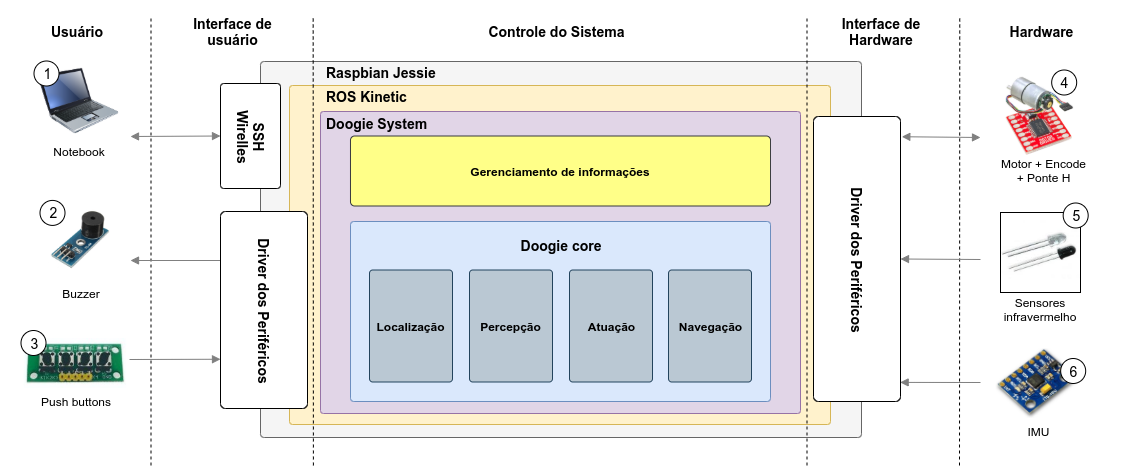
\includegraphics[width=1\textwidth]
	{Figures/arquitetura_geral}
	\label{fig:arquitetura_geral}
	\source{Própria Autoria}
\end{figure}

\subsection{Interface de usuário}
\label{ssec:interface_de_usuario}
O acesso à Raspberry Pi Zero é feito via SSH permitindo maior acessibilidade e segurança nos dados. O mesmo é feito remotamente através de conexão \textit{wireless}, possibilitando o acesso a linha de comandos da Raspberry bem como seu sistema de arquivos, de um outro computador.
 
O robô tem uma interface de interação com o usuário através de dois \textit{Push Buttons} e um \textit{Buzzer}. Os botões são utilizados para execução de tarefas tais como iniciar  e parar a execução da rotina principal do robô. O acesso a tais dispositivos é feito através do driver do periférico \gls*{gpio} que oferece \gls*{api} nas linguagens de programação Pyhton e C++.

\subsection{Interface de Hardware}
\label{ssec:interface_de_hardware}
O deslocamento do robô utiliza 2 motores de corrente contínua, acoplados à Encoders, possibilitando a obtenção de informações de posição e velocidade, com objetivo de otimizar o controle e acionamento dos motores. Além disso, para permitir que os motores girem em ambas as direções, são utilizados circuitos de ponte H.
 
Os sensores infravermelho são responsáveis por identificar obstáculos no trajeto do robô. Eles são dispostos de modo que o micromouse possa indentificar as paredes do labirinto à sua direita, esquerda e frente. Também é necessário auxílio da \gls*{imu} para obtenção de dados através dos sensores acelerômetro e giroscópio para estimar a posição com maior precisão. De forma similar a interface de usuário, serão utilizados drivers para estabelecer a comunicação entre o ambiente \gls*{ros} e o hardware acima descrito.

\subsection{Controle do sistema}
\label{ssec:controle_do_sistema}
A Raspberry Pi Zero é um mini computador de baixo custo e fácil acesso, capaz de reunir diversas funcionalidades em uma única placa de tamanho reduzido.  No mesmo, está instalado o sistema operacional Raspbian Jessie, possibilitando a utilização do \textit{framework} \gls*{ros}, responsável por gerenciar os subsistemas do robô.

Os principais subsistemas desenvolvidos para o Doogie foram:
\begin{itemize}
	\item \textbf{Localização:} o labirinto pode ser modelado em uma matriz, geralmente de tamanho 16x16. Esse subsistema tem o objetivo de prover informações sobre em qual posição dessa matriz o robô se encontra (linha e coluna);
	
	\item \textbf{Percepção:} com a utilização dos sensores infravermelho, o robô pode identificar se há obstáculos ao seu redor. Esse subsistema é responsável por informar se há obstáculos na frente, direita e/ou esquerda do mesmo;
	
	\item \textbf{Planejamento:} há diversas formas de mapear e completar o labirinto. Utilizando as informações obtidas dos outros subsistemas (localização e percepção), é possível realizar o algoritmo especificado e tomar as decisões necessárias para a realização da atividade;
	
	\item \textbf{Navegação:} subsistema responsável por gerenciar as ações de navegação do robô, tais como: ir para frente, virar para direita ou esquerda, parar, dentre outros.
	
	\item \textbf{Gerenciamento de Informações:} é o subsistema responsável por receber comandos através dos botões situados no chassi do robô e fornecer o mapa do labirinto a medida em que ele é percorrido. 
\end{itemize}

%--------- NEW SECTION ----------------------
\section{Especificação dos componentes}
\label{sec:especificacao_dos_componentes}
O robô Doogie é capaz de realizar de forma autônoma a procura do melhor caminho do labirinto que leva-o ao ponto de chegada. Uma vez descoberto, o robô percorre esse percurso no menor tempo possível. Para isso, o robô é composto de um sistema microprocessado compatível com distribuições Linux; sensores de percepção que permitem a detecção de obstáculos ao redor do robô; sensores de posição para o controle dos movimentos e localização dentro do labirinto; atuadores para permitir a locomoção de forma autônoma. Além disso, ele é equipado com bateria recarregável, conversor analógico/digital, multiplexador analógico, botões, LEDs e Buzzer. Os tópicos seguintes irão detalhar os principais componentes da plataforma móvel.

\subsection{Estrutura analítica do protótipo}
\label{ssec:pbs}
Para fornecer uma visão macro dos componentes que compõe o robô, foi elaborado um diagrama hierárquico, denominado \gls*{pbs}. Conforme Figura \ref{fig:pbs}, é possível visualizar a dependência entre os subsistemas e os componentes do robô. Além disso, diferente da Figura \ref{fig:arquitetura_geral}, esse diagrama oferece maior detalhamento dos elementos que estão relacionados a cada subsistema do robô.

\begin{figure}[H]
	\centering
	\caption{\textit{Prototype Breakdown Structure} do Doogie Mouse}
	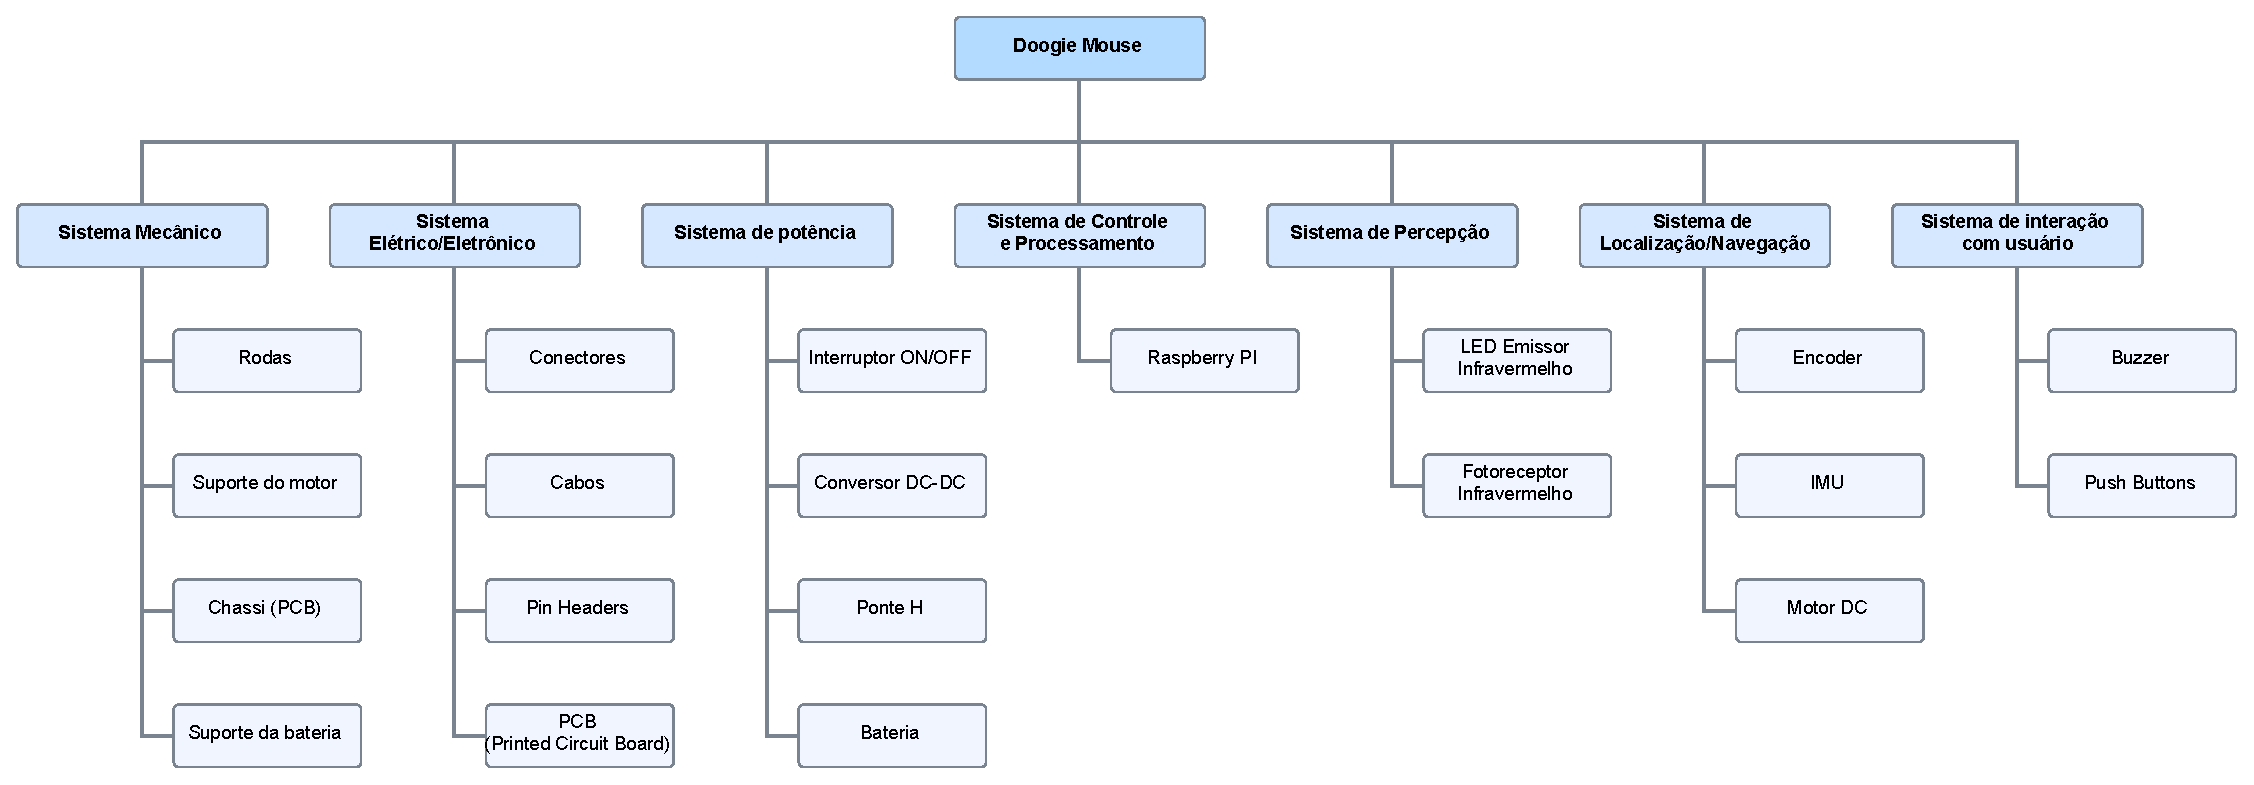
\includegraphics[width=1\textwidth]
	{Figures/prototype_breakdown_structure}
	\label{fig:pbs}
	\source{Própria Autoria}
\end{figure}

\subsection{Raspiberry Pi Zero W v1.1}
\label{ssec:raspiberry_pi_zero}
Para que o robô realize a resolução do labirinto, é necessário que ele contenha uma unidade de processamento central. Este dispositivo tem como objetivo, a partir dos dados dos sensores e de um algoritmo de resolução de labirintos, inferir qual o melhor conjunto de movimentos que permita o robô alcançar o ponto de chegada do labirinto no menor tempo possível. Como o modelo de robô Micromouse possui um baixo nível de abstração de \textit{hardware}, é necessário também que a unidade de processamento disponibilize periféricos necessários para a comunicação com os componentes do sistema. Não menos importante, a unidade deve possuir compatibilidade com o \textit{framework} \gls*{ros}, \textit{middleware }escolhido para o gerenciamento dos subsistemas que compõem o robô.

Portanto, foi escolhido o mini computador Raspberry PI Zero W v1.1: uma placa de baixo custo e com tamanho reduzido (apenas 6,5 x 3 cm), ótimo para projetos compactos como o robô Doogie. Esta placa é equipada com um processador \textit{single-core} Broadcom BCM2835 que opera na velocidade de 1 GHz aliado a uma memória RAM de 512 MB, além de um \textit{slot} para cartão microSD. A Raspberry PI Zero W v1.1 conta com \textit{WiFi} e \textit{Bluetooth} integrados, conector de vídeo mini HDMI e 2 portas USB para conectividade. Além disso, a placa permite que distribuições Linux como o Raspbian e Ubuntu sejam instaladas, as quais são compatíveis com \textit{framework} \gls*{ros}. A Raspberry Pi oferece também \glspl*{api} nas linguagens de programação Pyhton e C++ para controle do seu periférico \gls*{gpio} de 40 pinos. Essas interfaces permitem a utilização de protocolos de comunicação como UART, SPI e I2C; controle de motores através de saídas \gls*{pwm}; e pinos de entrada e saída para conexão com elementos digitais.

\subsection{Motor, Encoder e ponte H}
\label{ssec:motor_encoder_ponte-h}
Os robôs utilizados, em sua maioria, nas competições de Micromouse, têm como princípio de construção os robôs diferenciais. Este tipo de robô, muito comum no campo da robótica móvel, possui duas rodas conectadas a dois motores lateralmente opostos, os quais podem ser controlados independentemente. O sentido de giro e as velocidades das rodas determinam  o movimento do robô. Na especificação dos motores a serem utilizados em um robô diferencial, os parâmetros mais relevantes são sua velocidade e seu torque. Em casos de robôs providos por baterias, o consumo do motor e a tensão de alimentação são também fatores primordiais na sua escolha.

O controle utilizado em robôs diferenciais se baseia no modelo cinemático do mesmo, o qual inclui parâmetros construtivos dos robôs e, principalmente, as velocidades das rodas. Por isso, é necessário que além do motor, dois componentes estejam presentes na construção de um robô diferencial: um sensor de velocidade acoplado a cada roda, comumente utilizado um Encoder para tal função e um \textit{driver} de potência que permita controlar os motores de forma independente, isto é, controlar a velocidade e o sentido de giro de cada atuador.

Deste modo, o motor escolhido foi o \textit{Micro Metal Gearmotor HP 6V with Extended Motor Shaft} do fabricante Pololu. Para compatibilização, este fabricante fornece alguns componentes que podem ser comprados em conjunto com o motor. Assim, optou-se por utilizar o Encoder magnético desenvolvido para ser acoplado ao motor especificado, o qual possui uma resolução de 12 \gls*{cpr} e faixa de operação de tensão entre 2,7 V até 18 V. Além do Encoder, foi utilizado o par de rodas de 32 x 7 mm e os elementos de fixação também disponibilizados pelo mesmo fabricante. As especificações técnicas do motor podem ser visualizadas na Tabela \ref{tab:especificacao_do_motor}

\begin{table}[H]
	\centering
	\captionsetup{justification=centering}
	\caption{Especificações técnicas do motor \textit{Micro Metal Gearmotor HP 6V with Extended Motor Shaft}}
	\label{tab:especificacao_do_motor}
	\begin{tabular}{c|c}
		\hline
		\textbf{Descrição} & \textbf{Valor} \\ \hline
		Tensão & 6 V \\ \hline
		Tamanho & 10 x 12 x 26 mm \\ \hline
		Peso & 9,5 g \\ \hline
		Diâmetro do eixo & 3 mm \\ \hline
		Relação de redução & 29,86:1 \\ \hline
		Velocidade sem carga & 1000 RPM \\ \hline
		Corrente sem carga & 0,07 A \\ \hline
		Corrente com eixo parado & 1,6 A \\ \hline
		Torque com eixo parado & 0,57 kg.cm \\ \hline
		Máxima potência de saída1 & 1,5 W \\ \hline
		Máxima eficiência & 41 \% \\ \hline
		Velocidade na máxima eficiência & 830 rpm \\ \hline
		Torque na máxima eficiência & 0,10 kg.cm \\ \hline
		Corrente na máxima eficiência & 0,36 A \\ \hline
		Potência de saída na máxima eficiência & 0,89 W \\ \hline
	\end{tabular}
\end{table}

Para a ponte H, foi escolhido o módulo TB6612FNG, o qual permite o controle independente de dois motores de corrente contínua operando com tensão entre 4,5 à 13,5 V e com valores de corrente de até 1 A por canal. Não menos importante, este driver possui tensão lógica de operação entre 2,7 à 5,5 V e 100 kHz como máxima frequência de \gls*{pwm} permitida.

\subsection{Emissor e fotorreceptor Infravermelho}
\label{ssec:emissor_e_fotoreceptor_ir}
Os robôs da modalidade micromouse têm como funcionalidade essencial a percepção. Para que o sistema que controla  o robô decida qual a melhor opção de movimento, é necessário primeiro que se conheça quais as possibilidades existentes. Quem fornece informações para que essas possibilidades sejam criadas é exatamente a funcionalidade de percepção. O princípio básico dessa funcionalidade  é informar, para cada célula do labirinto, quantas paredes circundam-a e onde estes obstáculos se encontram (Norte, Sul, Leste e Oeste).

De acordo com as regras estabelecidas nas competições reguladas pelo \gls*{ieee} Região 9, os labirintos devem possuir cores específicas para os elementos que o compõe. Para as paredes do labirinto, a cor utilizada é a branca. A cor branca, quando comparada a cores mais frias, possui um alto valor de reflectância de luz cujo o comprimento de onda esteja dentro da faixa do infravermelho. Os sensores mais indicados que se beneficiam dessa característica são aqueles em que há alteração de propriedades física quando exposto a luz infravermelha. Sendo assim, a utilização de LEDs que operam com espectros não visíveis, como o infravermelho, em conjunto com fototransistores, é uma ótima opção para equipar robôs da modalidade micromouse.

Portanto, para instrumentar o projeto em questão, optou-se pela utilização do LED IR333C do fabricante Everlight, o qual opera na região do infravermelho, permitindo a emissão de luz com comprimento de onda de $940 \pm 45$ nm e com potência de dissipação e corrente máxima iguais a 150 mW e 100 mA respectivamente, ambas à temperatura ambiente. Para o receptor infravermelho, especificou-se o fototransistor PT333-3B do mesmo fabricante Everlight. Este sensor opera na faixa de espectro entre 840 a 1100 nm, possuindo maior sensibilidade quando exposto a ondas com comprimento de onda igual a 940 nm. À temperatura ambiente, o PT333-3B pode dissipar até 75 mW e drenar no seu coletor valores de correntes até 20 mA. Ambos componentes possui tensão de operação compatível a utilizada no robô Doogie. Vale ressaltar que estes componentes podem ser substituídos por similares desde que as características física e elétrica mencionadas sejam compatíveis.

\subsection{IMU}
\label{ssec:imu}
Os labirintos utilizados nas competições oficiais de Micromouse são formados por células de 18 x 18 cm. A estrutura física do labirinto é igual a uma matriz cuja a dimensão é 16 x 16. Sendo assim, os robôs devem saber em qual célula do labirinto ele se encontra no momento para coletar algumas informações, utilizadas posteriormente para a sua movimentação e para a otimização da solução do labirinto. Uma técnica utilizada para obter a posição do robô dentro do labirinto é a de Odometria. Nesta estratégia, a partir das informações do Encoder e das dimensões das rodas utilizadas, estima-se a distância percorrida em um intervalo de tempo, entretanto, é uma técnica vulnerável a erros acumulativos. Uma forma utilizada para melhorar a precisão deste método é a incorporação de uma \gls*{imu}, as quais têm seus dados fundidos com os dados da Odometria, resultando em uma medição mais confiável.

Isto posto, o robô Doogie foi equipado com a MPU-6050. Este sensor permite medição de aceleração e velocidade angular nos 3 eixos cartesianos, totalizando 6 graus de liberdade (6DOF), com a medição de cada canal disponibilizada por conversores \gls*{ad} com resolução de 16 bits. Além disso, a MPU-6050 realiza medição de temperaturas entre -40 à 85 \textdegree C possui interface de comunicação I2C e pode operar com tensões entre 3 à 5 V. Por im, algumas bibliotecas são disponibilizadas pela comunidade \textit{open source} para comunicação com este dispositivo nas linguagens de programação Python e C++.

\subsection{Conversor Analógico/Digital e Multiplexador Analógico}
\label{conversor_multiplexador_analogico}
Como descrito no tópico \ref{ssec:raspiberry_pi_zero}, a Raspberry Pi Zero W v1.1 possui 40 pinos digitais. Entretanto, nenhum deles é habilitado para fazer conversão \gls*{ad}. Como os sensores infravermelho especificados (ver tópico \ref{ssec:emissor_e_fotoreceptor_ir}) fornecem valores analógicos de tensão em sua saída, é necessário o uso de um conversor externo. Além disso, robôs autônomos necessitam de verificação periódica da autonomia de sua bateria. Essa informação é também obtida de forma analógica. Logo, torna-se necessário que o Doogie Mouse seja equipado com um conversor \gls*{ad} externo.

Mediante o exposto, foi selecionado o conversor ADS1115. Esse conversor funciona com tensões entre 2 à 5,5 V, e a tensão máxima nos pinos analógicos é igual à tensão de alimentação. Os pinos analógicos podem ser programados como 4 pinos independentes, ou dois canais diferenciais. Ademais, a interface de comunicação utilizada pelo ADS1115 é I2C.

O ADS1115 possui apenas 4 canais, entretanto, são necessários 5 canais: 4 para os sensores infravermelho e um para bateria. Para solucionar a carência de canais, foi especificado o multiplexador analógico 74HC4051. Esse módulo pode multiplexar até 8 canais, permitindo tensões de 2 à 10 V e frequência de até 170 MHz.

\subsection{Lista de componentes}
\label{ssec:bom}
A lista contendo todos os componentes bem como suas respectivas quantidades e descrição pode ser visualizada no Apêndice \ref{apend:bom} deste documento.

%--------- NEW SECTION ----------------------
\section{Modelo mecânico}
\label{sec:modelo_mecanico}

\subsection{Plataforma Robótica}
\label{ssec:plataforma_robotica}

Para o design do robô, foi utilizado como um ponto de partida o TON-BOT v1.1, plataforma desenvolvida pela Ioton Technology \cite{ioton}. Além disso, conforme ítem 7 da subseção \ref{sec:requisitos_do_projeto}, ele deve ter suas dimensões não superiores à uma seção retangular de 15 x 15 x 10 cm.

A partir dessas premissas e da análise feita na subseção \ref{sec:requisitos_do_projeto}, buscou-se um design mecânico simples e de maior leveza. Dessa forma, foi utilizado como \textit{frame} do robô as próprias \glspl*{pci}, buscando posicionar suas rodas de forma a mantê-las alinhadas ao centro de massa de todo o conjunto mecânico. Para tanto, uma modelagem em \gls*{cad} inicialmente foi realizada através da ferramenta Solidworks, buscando iterativamente a melhor disposição de seus elementos físicos (rodas, sensores e demais componentes eletrônicos das placas), para a elaboração das \glspl*{pci}, vistas na subseção \ref{ssec:esquematicos_eletronicos}. Assim elaborou-se um esboço do modelo mecânico conforme a Figura \ref{fig:doogie_boards_3d}.

\begin{figure}[H]
	\centering
	\caption{Modelo 3D do Doogie Mouse}
	\subfigure[Representação 3D da placa inferior]{\label{fig:doogie_bottom__board_3d}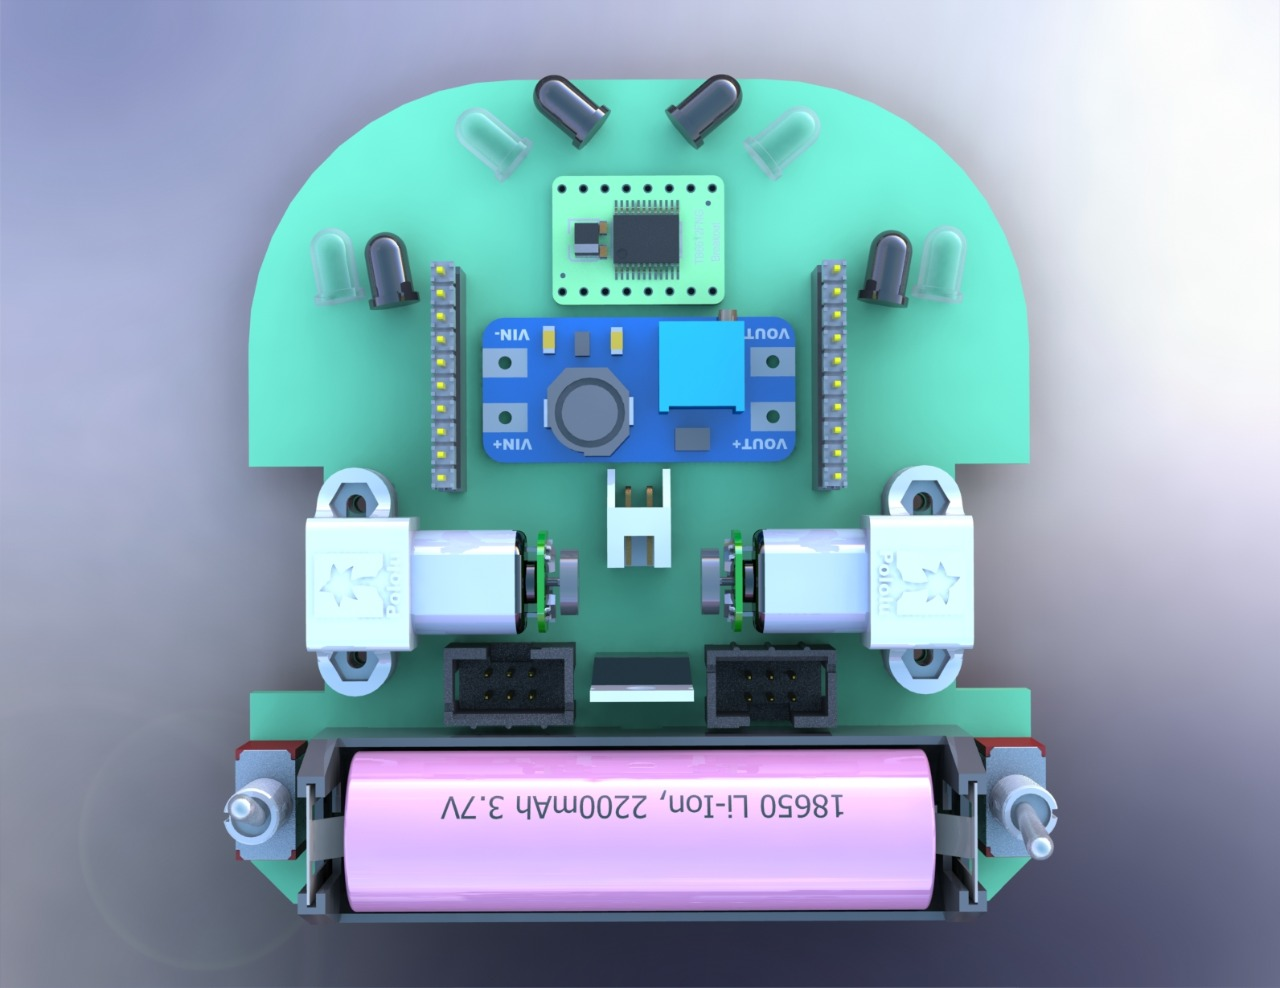
\includegraphics[scale=0.15]{doogie_bottom_board_3d.jpeg}}
	\subfigure[Representação 3D da placa superior]{\label{fig:doogie_top_board_3d}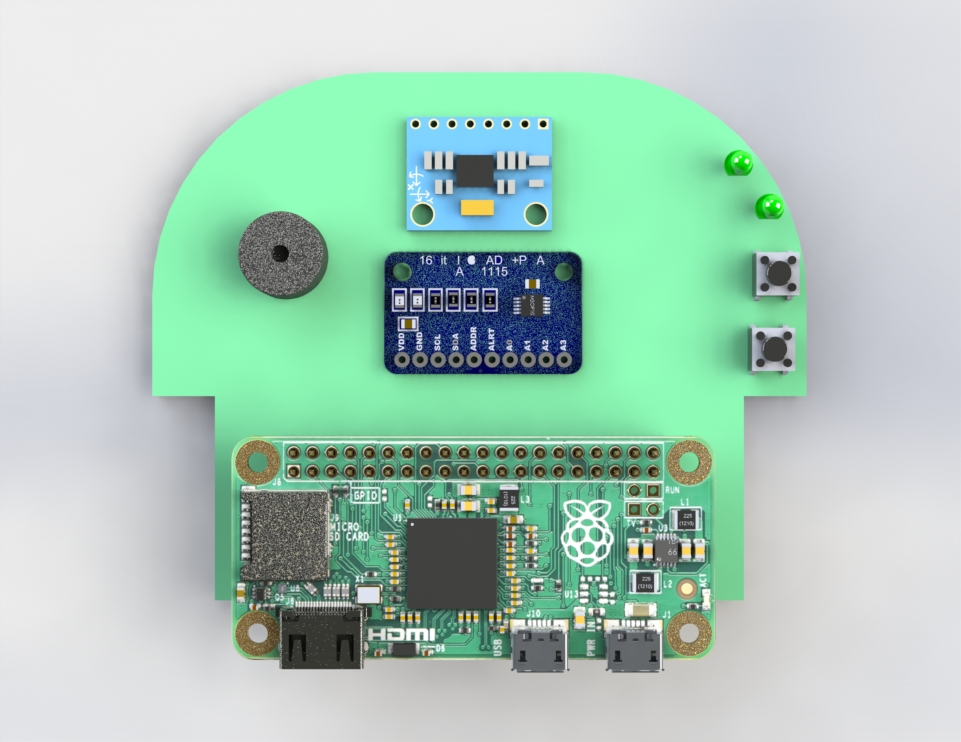
\includegraphics[scale=0.2]{doogie_top_board_3d.jpeg}}
	\subfigure[Modelo 3D do Doogie Mouse]{\label{fig:doogie_3d}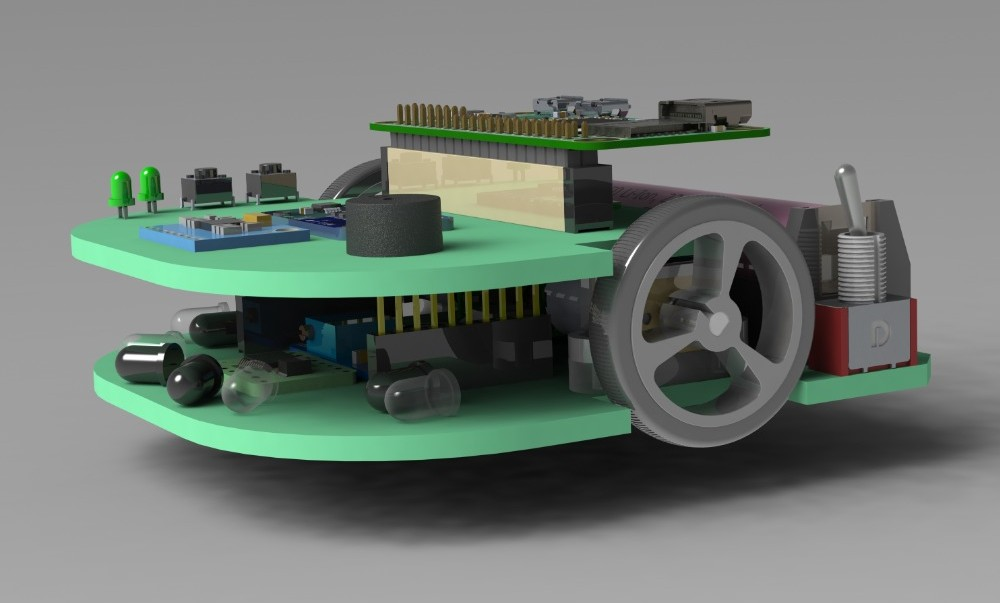
\includegraphics[scale=0.38]{doogie_3d.jpeg}}
	\label{fig:doogie_boards_3d}
	\source{Própria Autoria}
\end{figure}

Da esquerda para direita visualiza-se as placas inferior, superior e o modelo completo do robô visto em perspectiva. A placa inferior possui 98 mm de comprimento e 92,90 mm de largura, enquanto a placa superior possui 75 mm de comprimento e 92,90 mm de largura. Foi necessário o uso de duas placas para melhor adequação dos componentes eletrônicos sem atrapalhar eventuais manutenções no dispositivo nem dificultar sua montagem. O modelo 3D final, renderizado, pode ser visto abaixo na Figura \ref{fig:doogie_boards_3d_render}. Os desenhos técnico da plataforma móvel podem ser visualizados no Apêndice \ref{apend:diagramas_mec_robo}.

\begin{figure}[H]
	\centering
	\caption{Modelo 3D Renderizado do Doogie Mouse}
	\subfigure[Modelo 3D Renderizado do Doogie Mouse]{\label{fig:doogie_3d_render}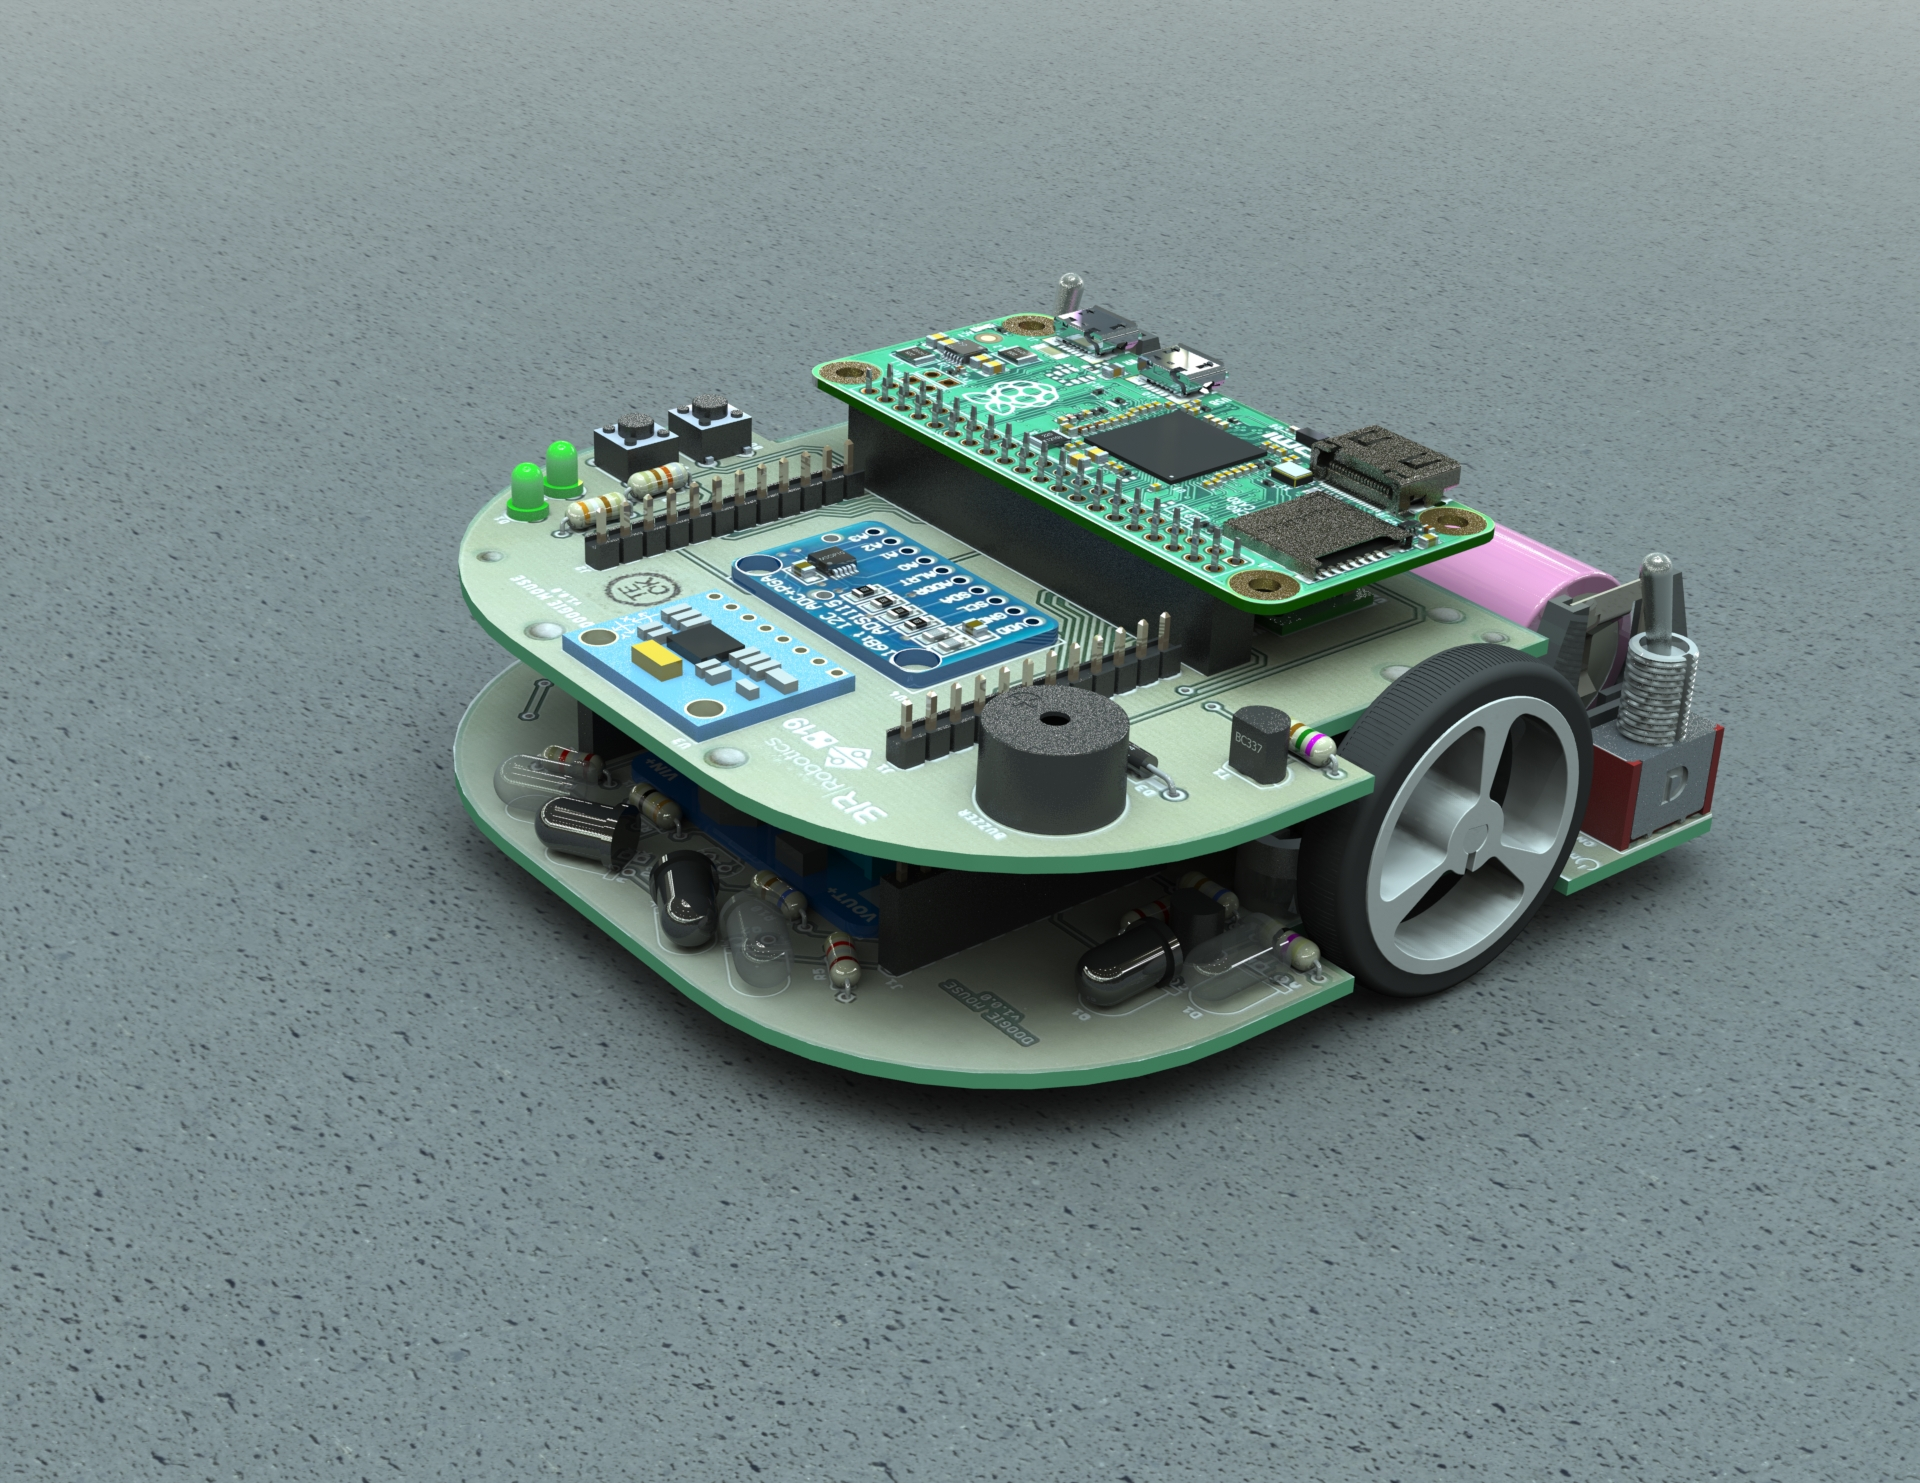
\includegraphics[scale=0.2]{Doogie_Mouse_Renderizado.JPG}}
	\subfigure[Vista frontal]{\label{fig:doogie_frontal_render}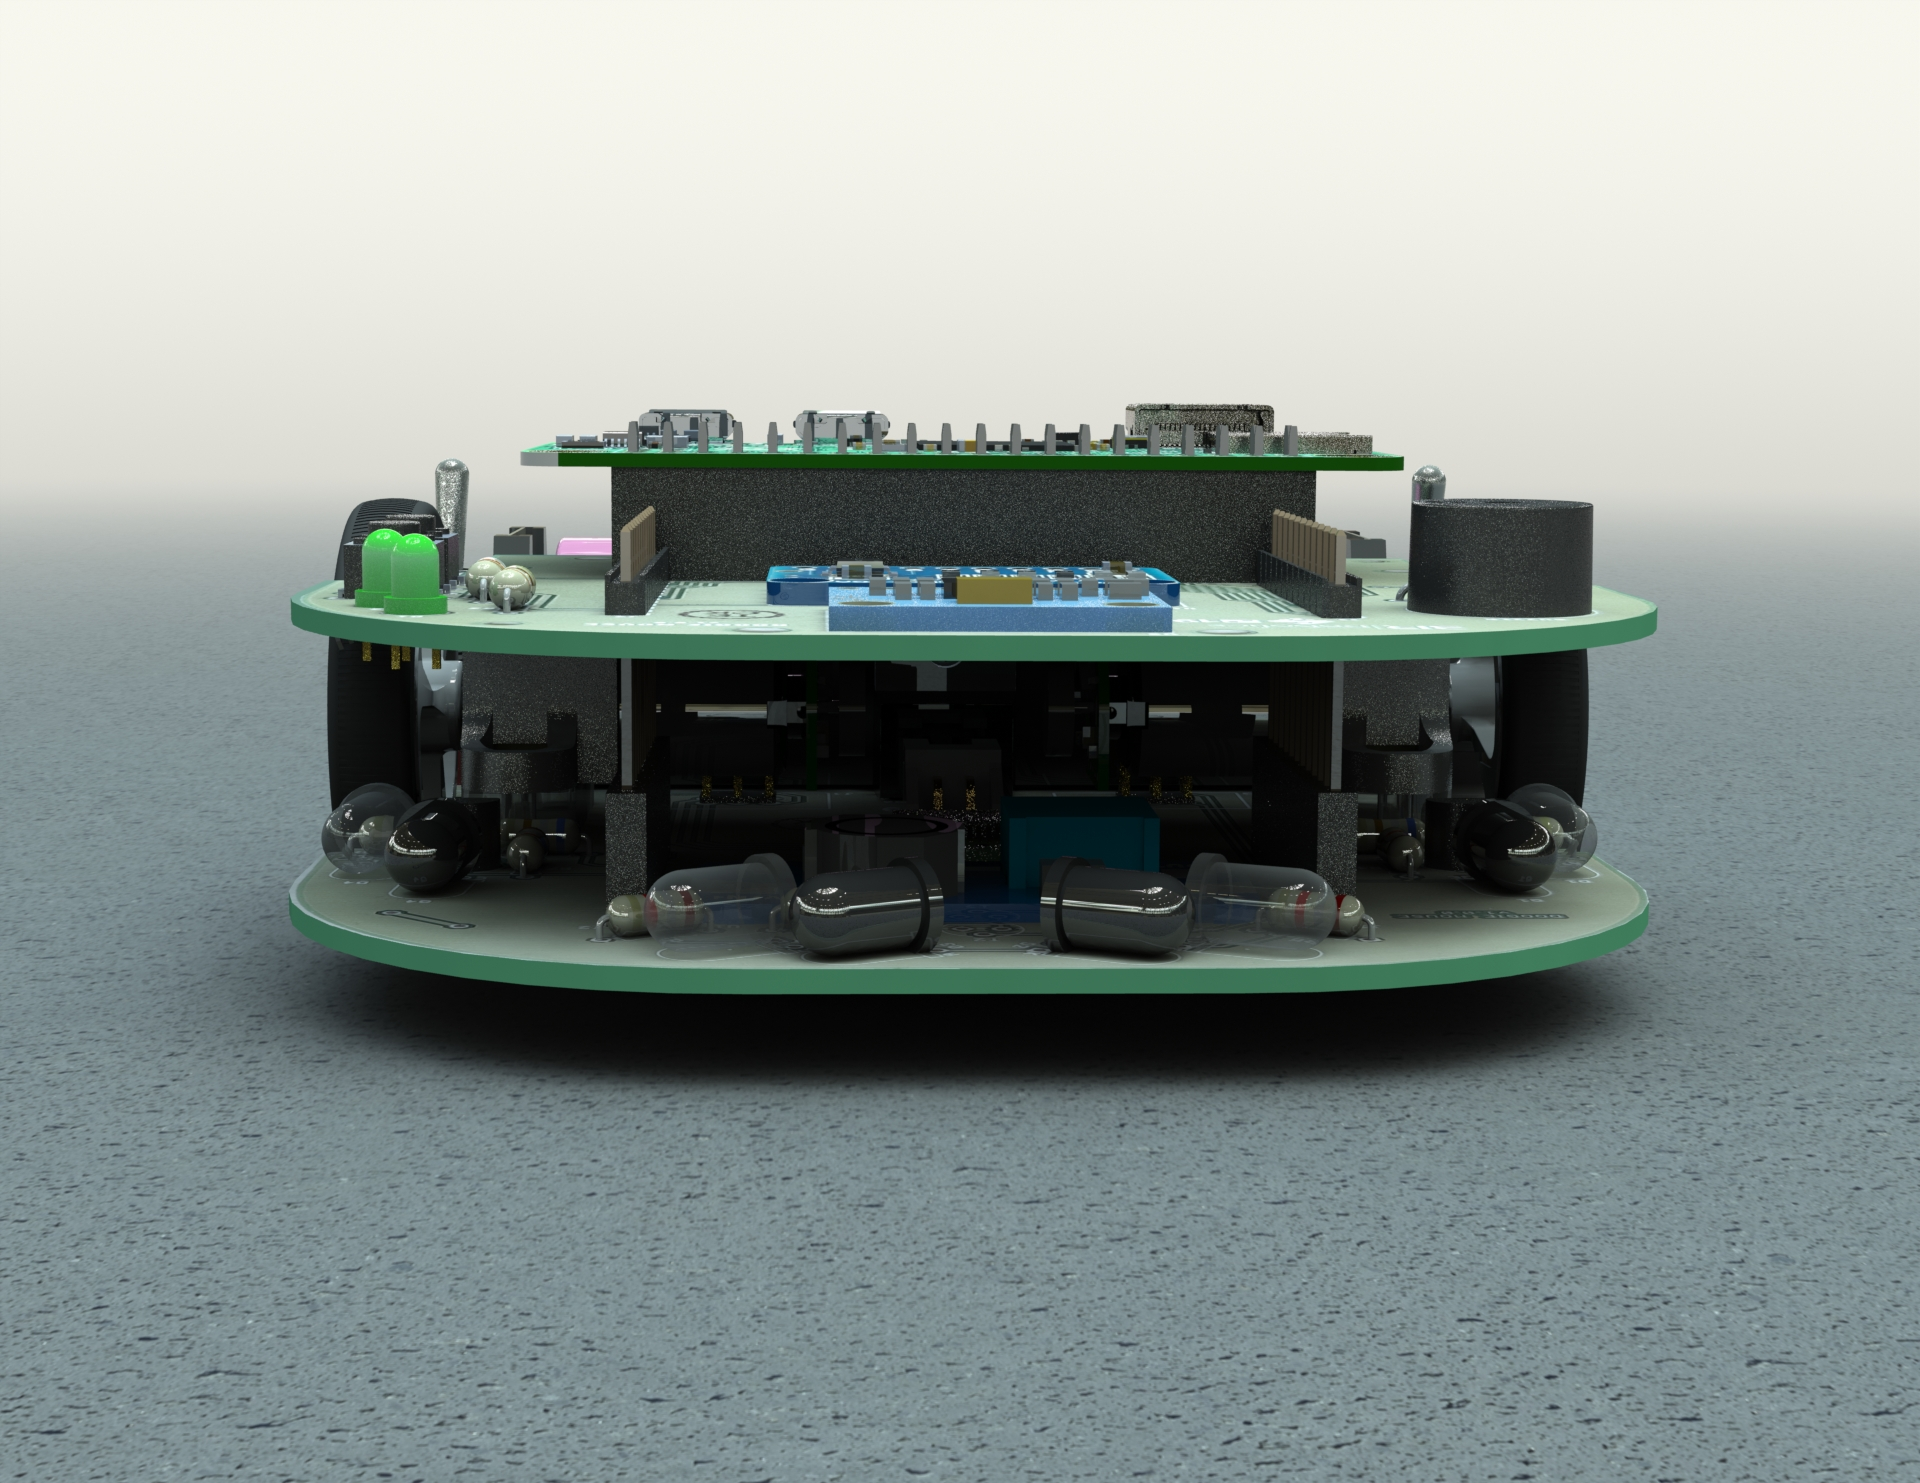
\includegraphics[scale=0.11]{Doogie_frontal_v4.JPG}}
	\subfigure[Vista Lateral]{\label{fig:doogie_lateral_render}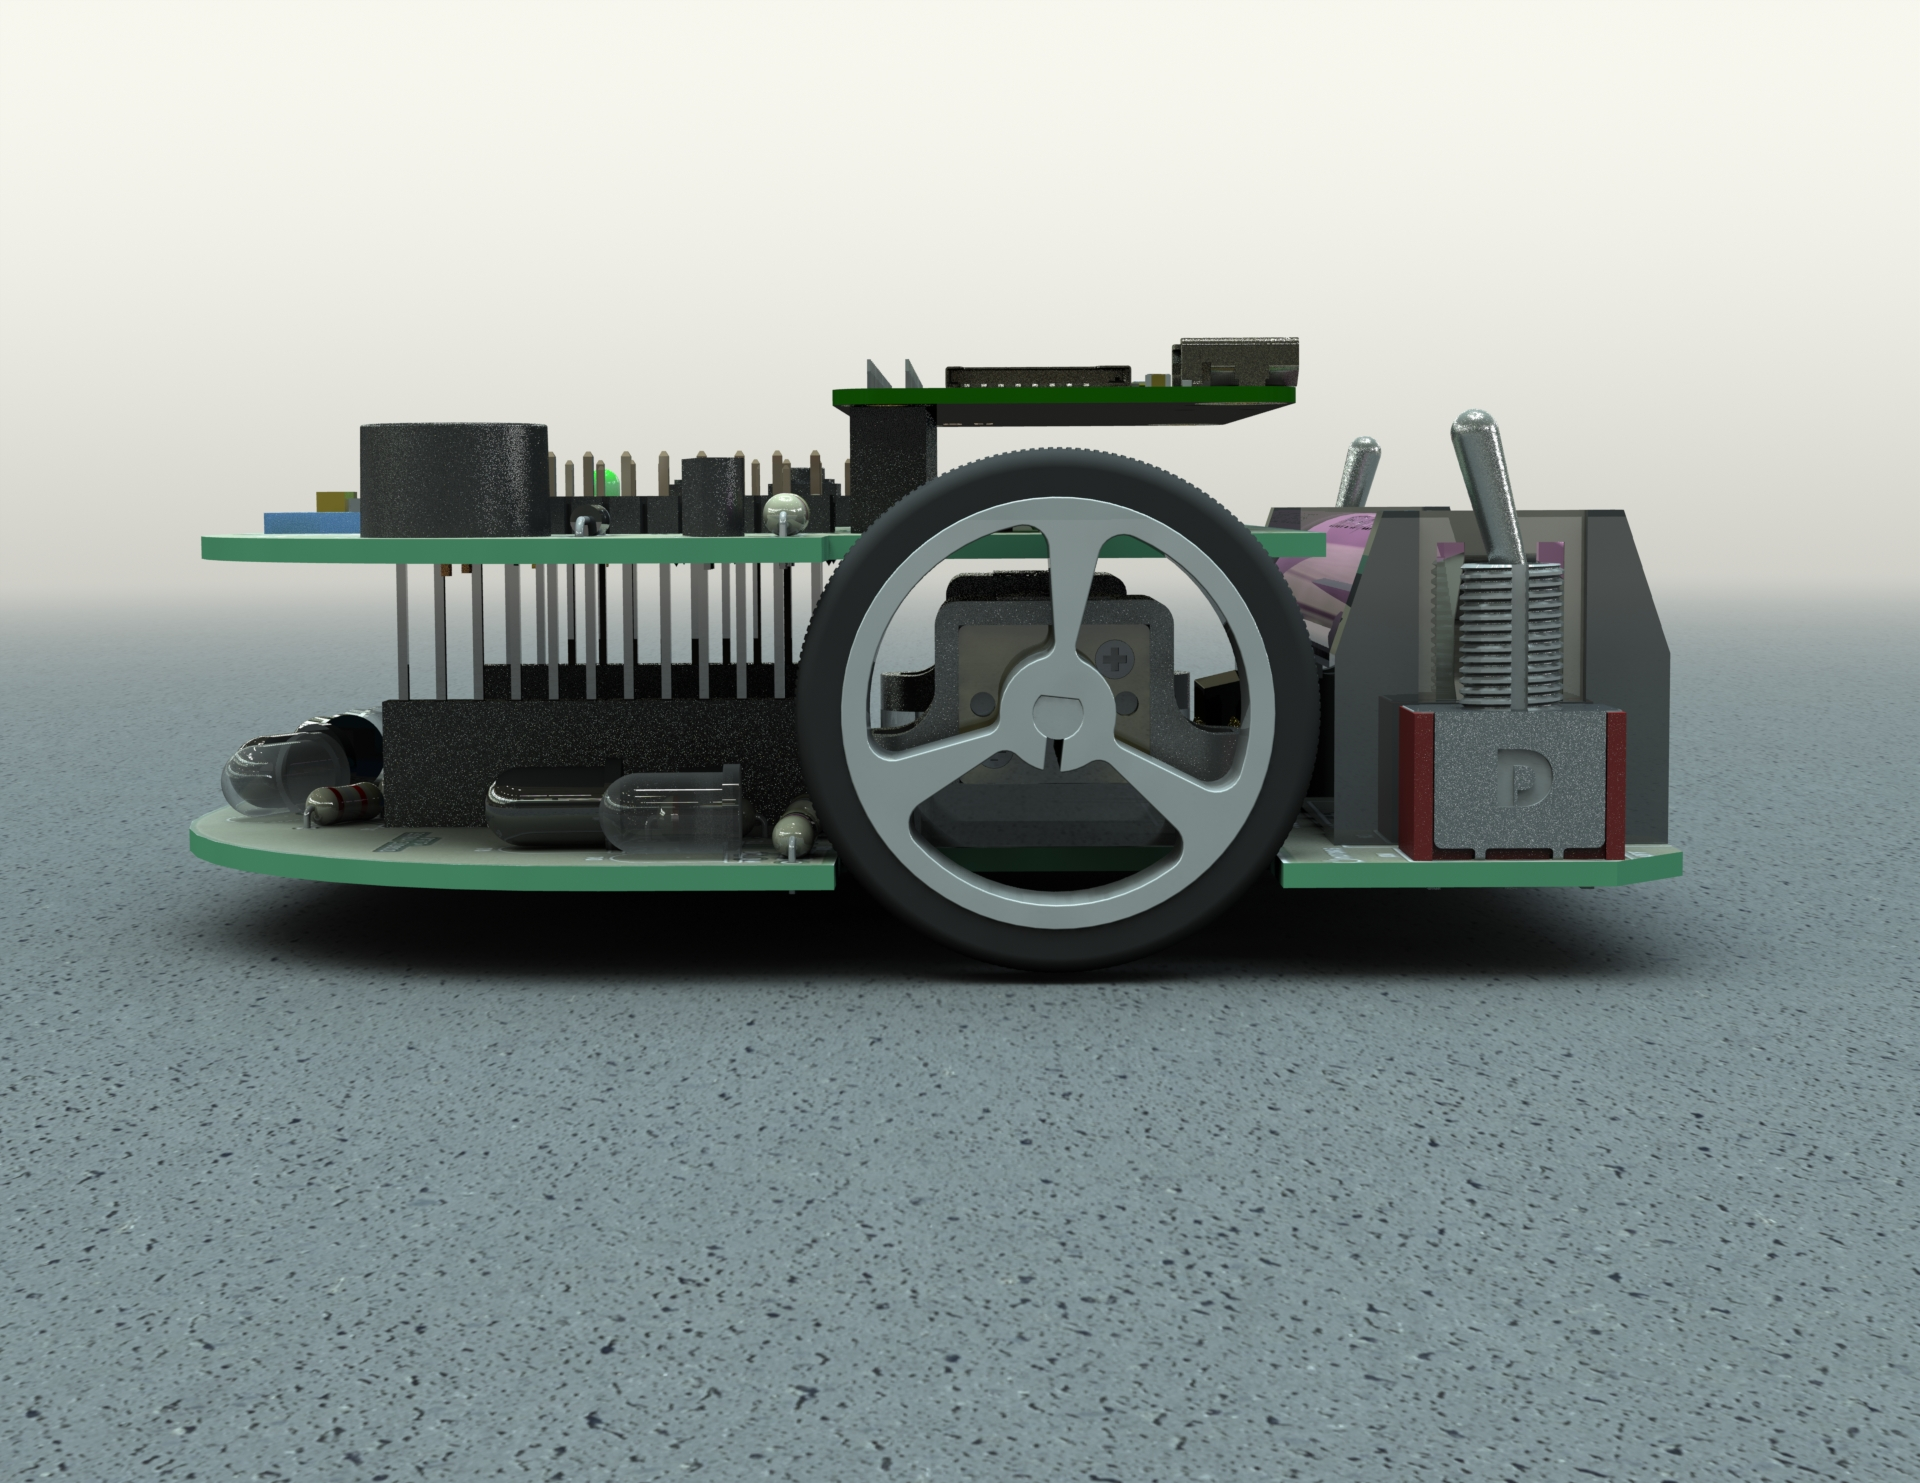
\includegraphics[scale=0.11]{Doogie_lateral_v4.JPG}}
	\label{fig:doogie_boards_3d_render}
	\source{Própria Autoria}
\end{figure}

\subsection{Labirinto}
\label{ssec:labirinto}

O modelo do labirinto foi desenvolvido a partir de uma adaptação do modelo IEEE \cite{Wan2019}. Por ser um labirinto protótipo, preferiu-se trabalhar com uma matriz de 10x10 células quadradas, em vez de 16x16, mantendo-se as mesmas dimensões da célula de 18 mm x 18 mm, com 50 mm de altura.

Além disso, buscou-se um design que fosse modular, de forma a facilitar seu transporte bem como múltiplas configurações do labirinto pela alteração da posição de suas paredes. Para isso, optou-se pela utilização de pivôs de madeira para a fixação das paredes na placa do labirinto, conforme visto na Figura \ref{fig:pivo}. Um exemplo de uma célula é mostrado na Figura \ref{fig:pivo}, enquanto seus desenhos técnicos se encontram no Apêndice \ref{apend:diagramas_mec_labirinto}.

\begin{figure}[H]
	\centering
	\caption{Modelo mecânico do labirinto}
	\subfigure[Pivô de fixação]{\label{fig:pivo}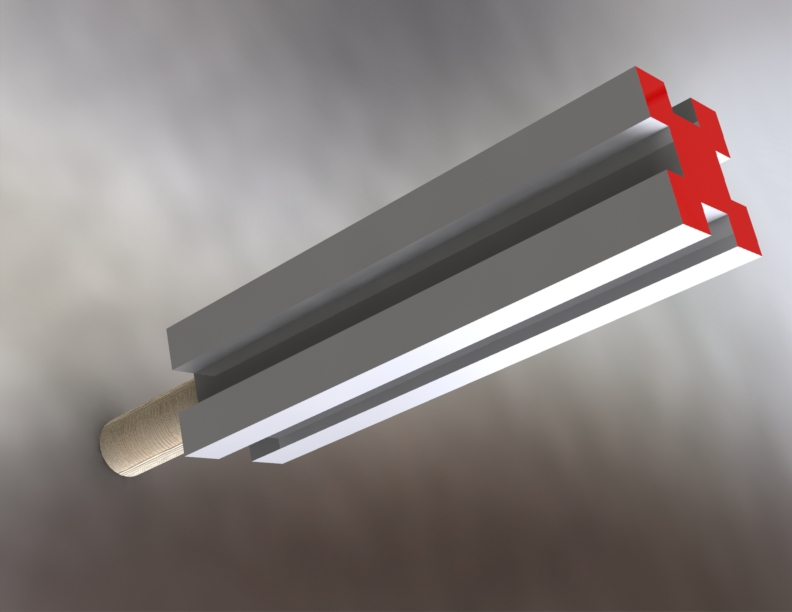
\includegraphics[scale=0.2]{Figures/pivo.JPG}}
	\subfigure[Célula do labirinto montada]{\label{fig:celula_labirinto}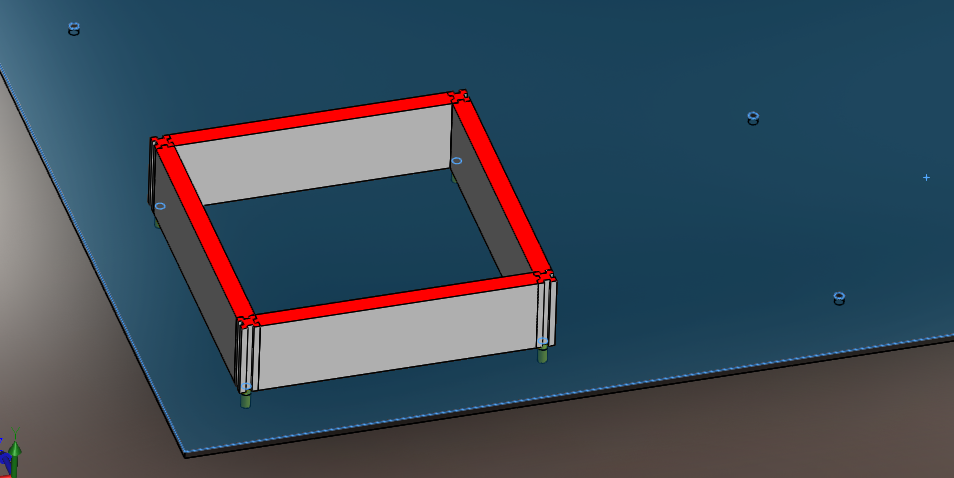
\includegraphics[width=0.54\textwidth]
		{Figures/maze_cell}}
	\label{fig:modelo_mecanico_labirinto}
	\source{Própria Autoria}
\end{figure}

%--------- NEW SECTION ----------------------
\section{Modelo esquemático de alimentação e comunicação}
\label{sec:arquitetura_eletrica_geral}
O Doogie é equipado com uma bateria do tipo Li-Ion com 3,6 V de tensão nominal. Para compatibilizar o nível de tensão da bateria com os demais componentes, são utilizados dois conversores DC-DC. O primeiro irá fornecer 6 V exclusivamente para os motores e os LEDs emissores. Já o segundo, é responsável por fornecer 5 V à Raspberry Pi. Entretanto, os componentes que estão conectados a Raspberry Pi são energizados com 3,3 V através de um conversor DC-DC interno a placa do sistema microprocessado.

Com intuito de facilitar a replicação do robô por usuários que queiram utilizá-lo, optou-se pelo uso de \textit{breakout boards}, que são placas eletrônicas pré-montadas. O Doogie possui seis delas: dois conversores de tensão DC-DC, um conversor \gls*{ad}, uma \gls*{imu}, um multiplexador analógico e uma ponte H. Os demais componentes como resistores, transistores, LEDs infravermelho, fototransistores e conectores, são soldados diretamente na \gls*{pci}.

Os componentes do Doogie se comunicam e são controlados de diversas formas. O conversor \gls*{ad} e a \gls*{imu} se comunicam com a Raspberry Pi através de um barramento I2C. Como o conversor \gls*{ad} especificado possui apenas 4 canais (um para cada sensor infravermelho), optou-se por utilizar um multiplexador analógico para permitir que o valor de tensão da bateria também seja obtido. Este multiplexador é controlado por pinos digitais da unidade de processamento. Por fim, o controle dos motores é realizado por uma ponte H com dois canais independentes. Esse \textit{driver} de potência permite que os sentidos de giros dos motores sejam controlados por pinos digitais da Raspberry Pi enquanto o controle de velocidade seja realizado por \gls*{pwm}.

A arquitetura elétrica na Figura \ref{fig:arquitetura_eletrica} demonstra como esses componentes descritos estão interligados eletricamente. A propósito de melhor visualização, o referencial de tensão (Ground - GND) foi omitido.

\begin{figure}[H]
	\centering
	\caption{Representação elétrica do Doogie Mouse.}
	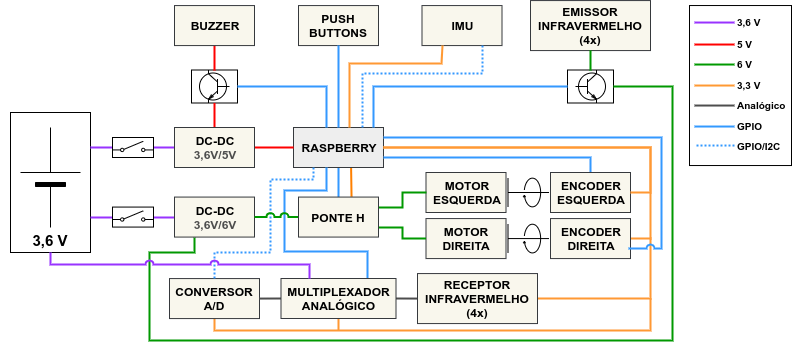
\includegraphics[width=1\textwidth]
	{Figures/arquitetura_eletrica}
	\label{fig:arquitetura_eletrica}
	\source{Própria Autoria}
\end{figure}

\subsection{Esquemáticos eletrônicos}
\label{ssec:esquematicos_eletronicos}
Como explicado no tópico \ref{sec:modelo_mecanico} o Doogie Mouse possui duas \glspl*{pci} que são utilizadas como chassi do robô. Além disso, como também citado na subseção \ref{sec:arquitetura_eletrica_geral}, os componentes eletrônicos e as \textit{breakout boards} são soldados diretamente na \gls*{pci}. Para elaboração do \textit{layout} de tais placas, foi utilizado o software Autodesk Eagle 9.4.2. O resutado obtido pode ser visualizado na Figura \ref{fig:doogie_boards}. Já os esquemáticos eletrônicos, que descrevem em maior detalhe as ligações elétricas entre todos os componentes do robô bem como o valor das grandezas físicas dos elementos eletrônicos, podem ser visualizados no Apêndice \ref{apend:diagramas_eletronicos} deste documento.

\begin{figure}[H]
	\centering
	\caption{\textit{Layout} das PCIs do Doogie Mouse}
	\subfigure[Placa inferior]{\label{fig:doogie_bottom_board}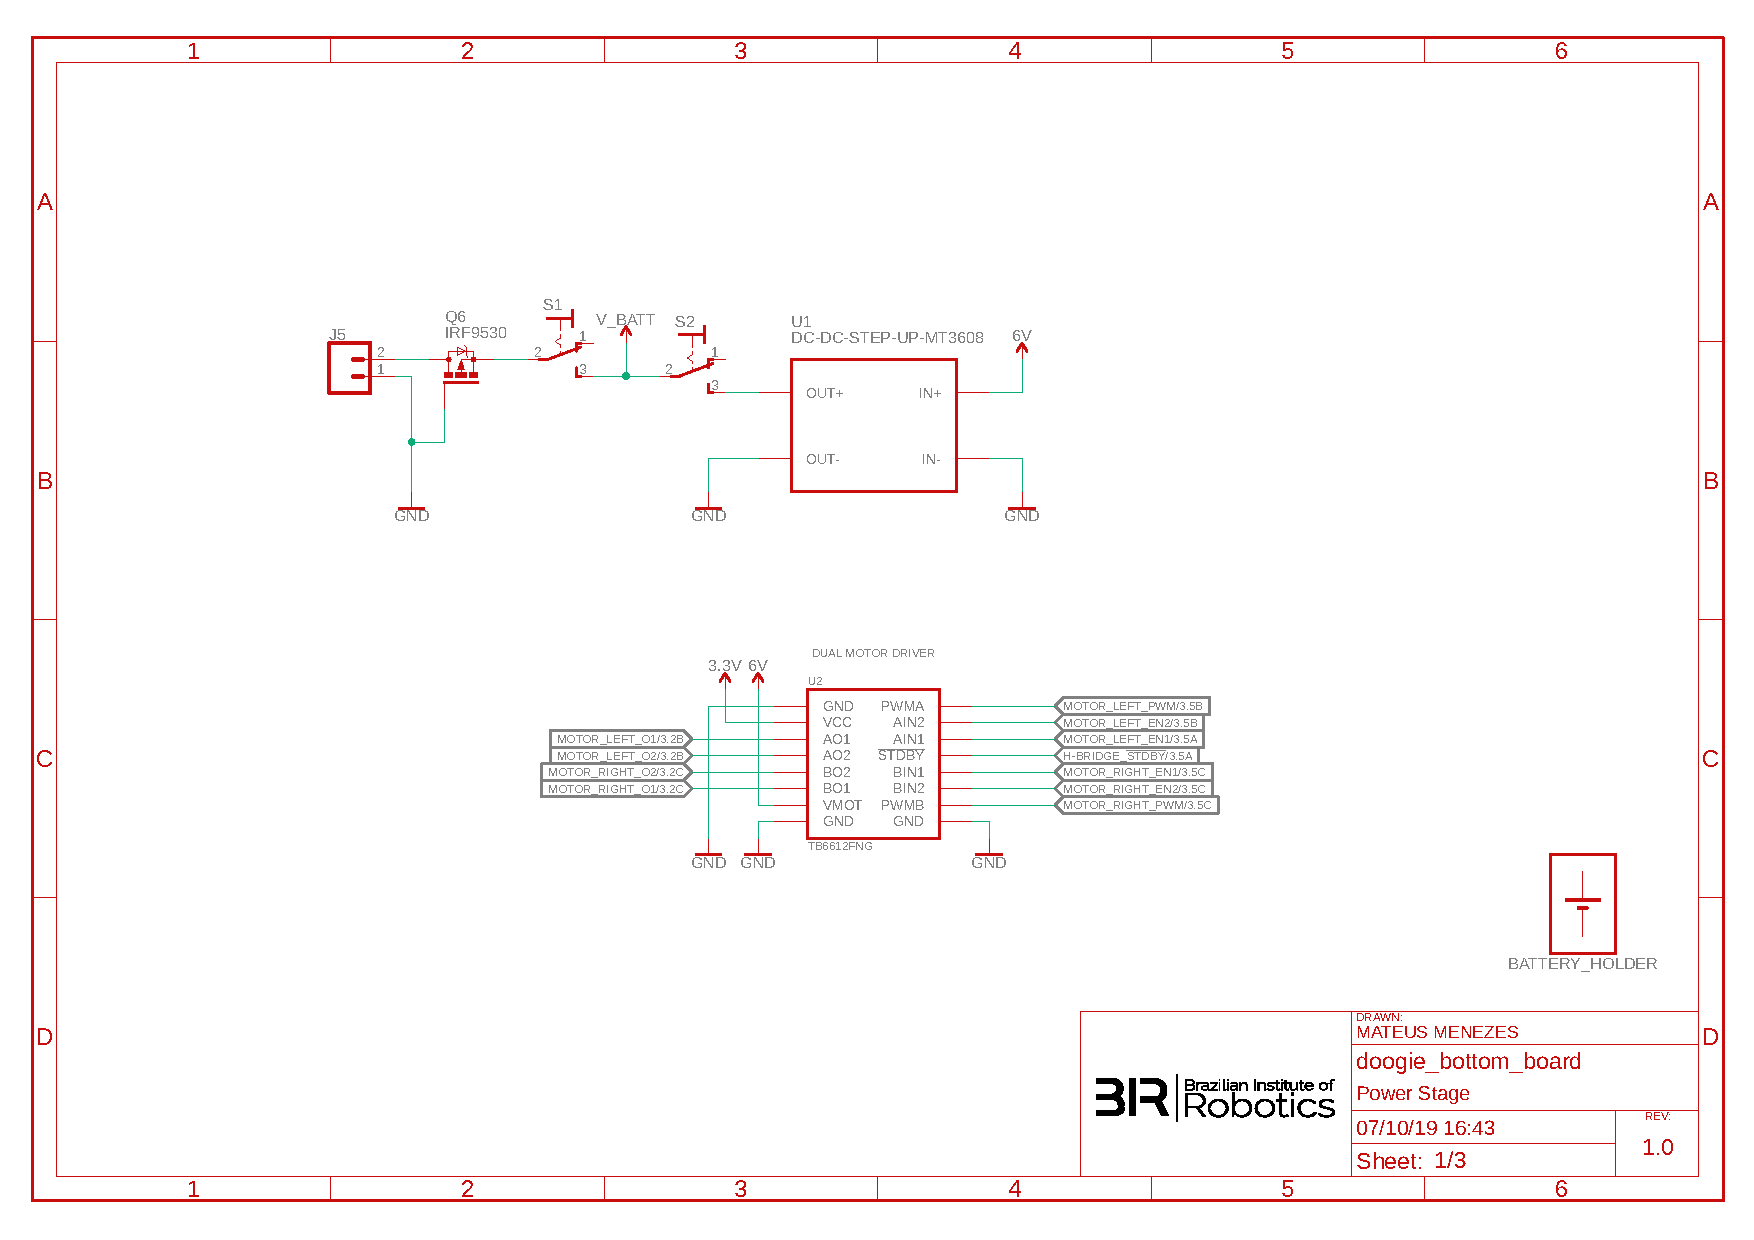
\includegraphics[scale=0.2]{doogie_bottom_board}}
	\subfigure[Placa superior]{\label{fig:doogie_top_board}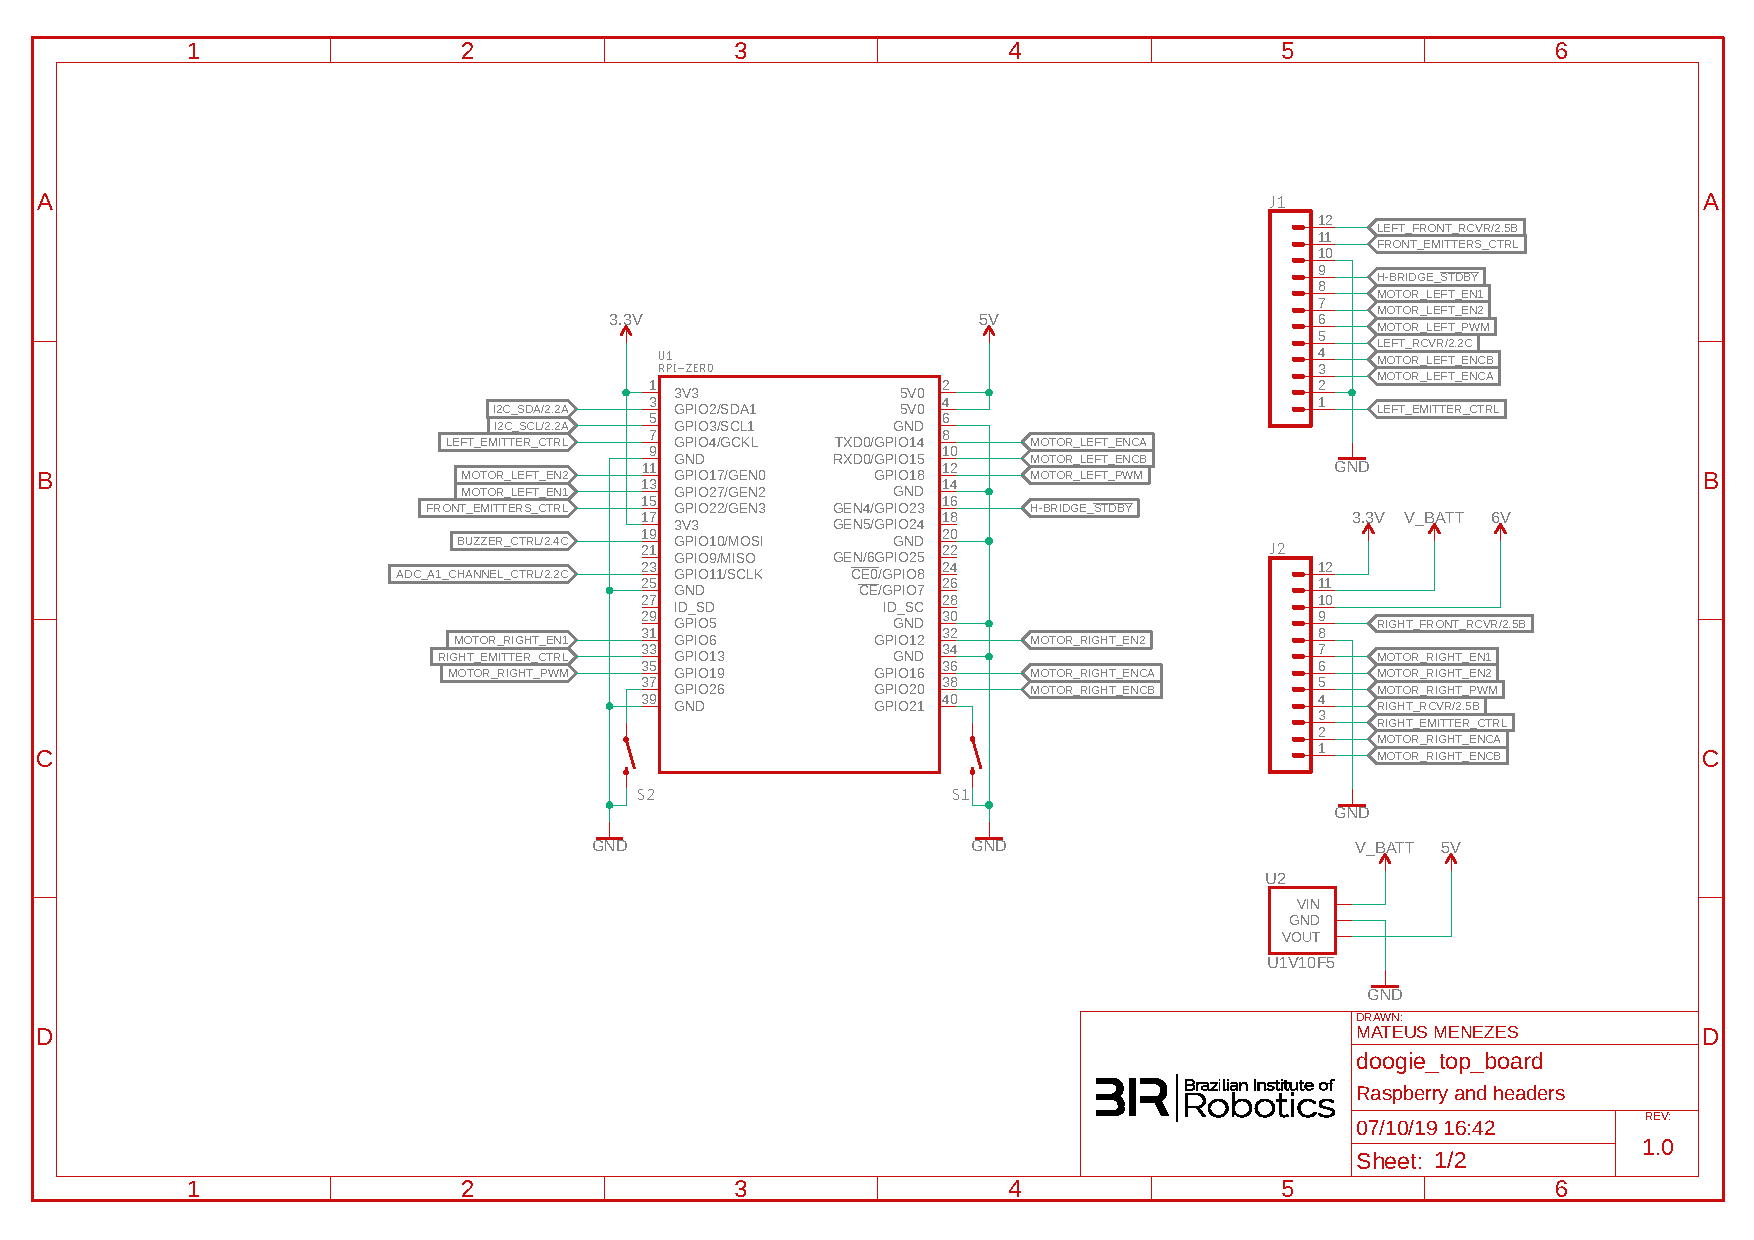
\includegraphics[scale=0.15]{doogie_top_board}}
	\label{fig:doogie_boards}
	\source{Própria Autoria}
\end{figure}

%--------- NEW SECTION ----------------------
\section{Especificação das funcionalidades}
\label{sec:especificacao_das_funcionalidades}
As funcionalidades de um robô descrevem os subsistemas e a lógica de operação dos mesmos. No Doogie, existem quatro funcionalidades principais: Localização, Percepção, Navegação e Usabilidade. O fluxo de informações de tais funcionalidades pode ser visualizado na Figura \ref{fig:especificacao_funcional_geral}. Observa-se nesse fluxograma como cada funcionalidade está interligada com as demais e quais informações são trafegadas entre elas. Para melhor entendimento, é descrito nos tópicos sequentes cada funcionalidade individualmente.

\begin{figure}[H]
	\centering
	\captionsetup{justification=centering}
	\caption{Fluxo de informações das funcionalidades Localização, Percepção, Navegação e Usabilidade.}
	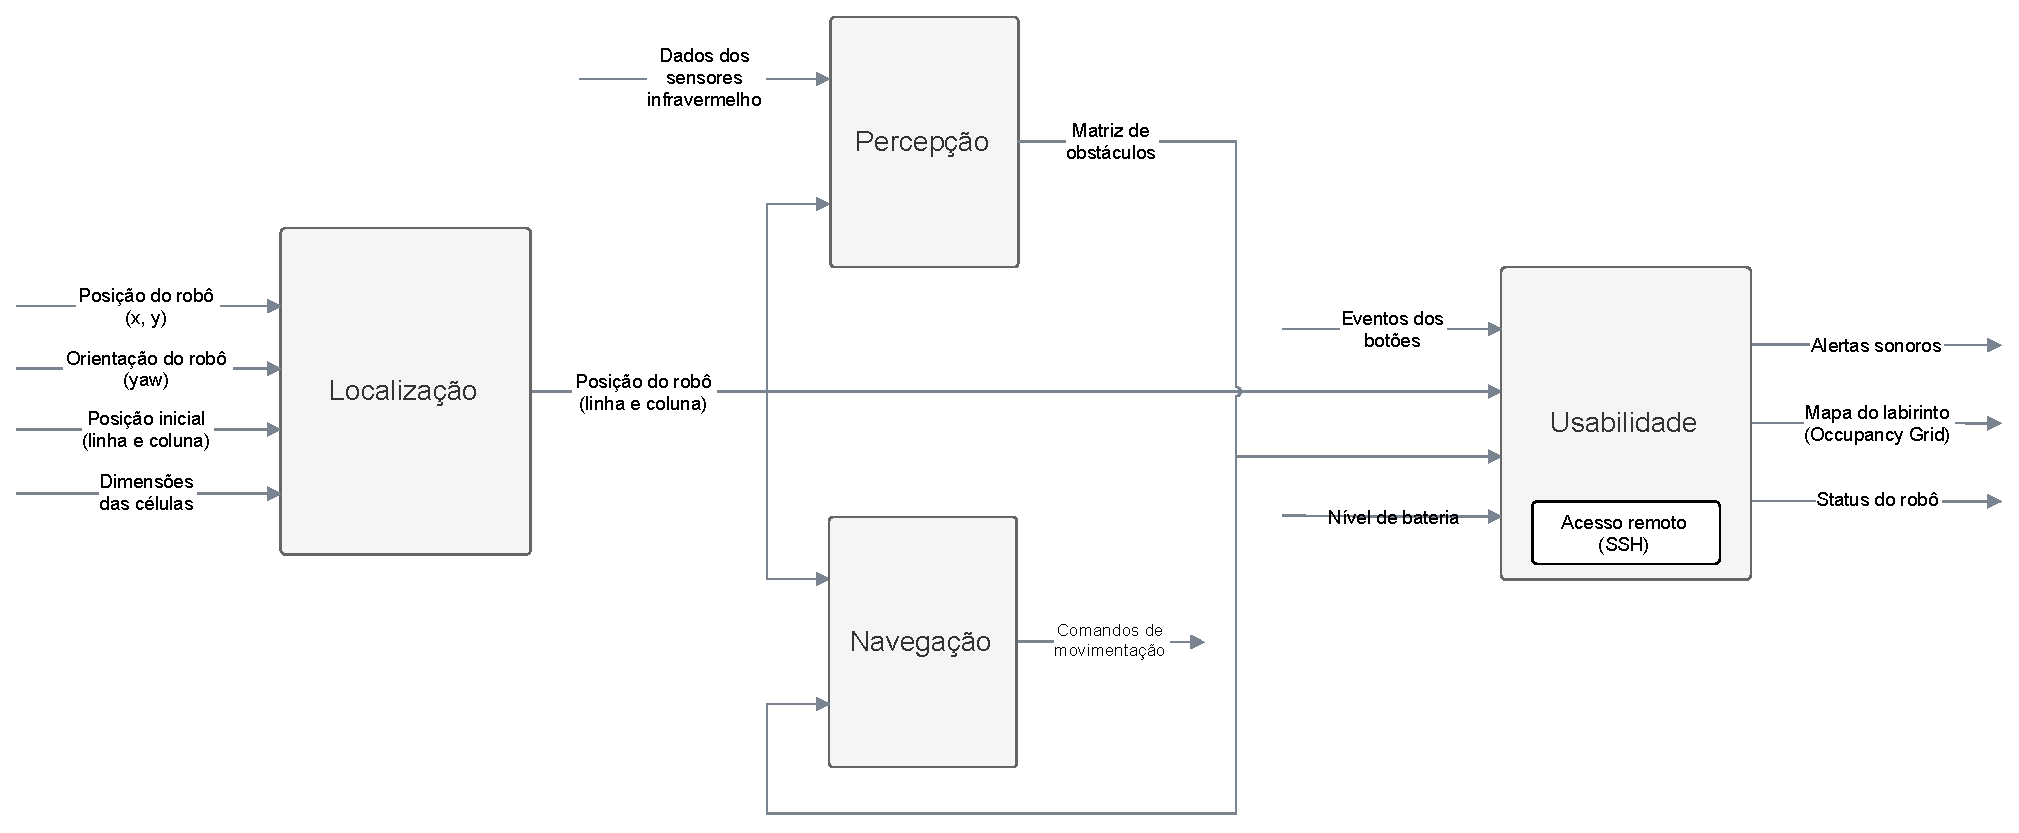
\includegraphics[width=1\textwidth]
	{Figures/especificacao_funcional_geral}
	\label{fig:especificacao_funcional_geral}
	\source{Própria Autoria}
\end{figure}

\subsection{Localização}
\label{ssec:funcionalidade_localizacao}
O labirinto a ser percorrido pelo micromouse será modelado como uma matriz 16 x 16, sendo dividido em células de largura e comprimento fixos. Para que o robô consiga decidir para onde ele deve ir, primeiro é necessário saber onde ele está.

A estratégia utilizada para a obtenção da posição do Doogie utilizará a técnica de Odometria, onde, a partir das informações do Encoder e das dimensões das rodas utilizadas, estima-se a distância percorrida em um intervalo de tempo. Além disso, para melhorar a precisão da medição, será utilizada uma \gls*{imu}, capaz de fornecer os dados de aceleração e velocidade angular nos três eixos cartesianos.

Uma vez que o robô consiga calcular a distância percorrida, em qualquer intervalo de tempo, sabendo as dimensões de cada célula e assumindo que seu ponto de partida foi informado, é possível determinar as coordenadas do mesmo dentro do labirinto: linha e coluna. 

\subsubsection{Objetivo}
Interpretar as informações fornecidas pela Odometria e identificar a posição do robô dentro do labirinto.

\subsubsection{Dependências}
Esse pacote depende da aquisição de dados publicados por:
\begin{itemize}
	\item Pacote de driver da \gls*{imu};
	\item Pacote de driver do motor.
\end{itemize}
	
\subsubsection{Premissas}
Para que essa funcionalidade alcance o seu propósito, assume-se que:
\begin{itemize}
	\item O ponto de partida do robô será informado pelo usuário: [linha, coluna];
	\item O valor de comprimento e largura das células são conhecidos pelo sistema e é diferente de zero;
	\item O valor de comprimento e largura (em metros) das células será previamente informado;
	\item O pacote de \textit{driver} da \gls*{imu}, aliado ao pacote de \textit{driver} do motor, oferecerão a informação de orientação do robô.
\end{itemize}

\subsubsection{Saídas}
Essa funcionalidade tem como saídas:
\begin{itemize}
	\item Doogie position: localização do robô na matriz, no formato: [linha, coluna].
\end{itemize}

A Figura \ref{fig:especificacao_funcional_localizacao} demonstra as entradas e saídas da funcionalidade em questão.

\begin{figure}[H]
	\centering
	\caption{Fluxograma ilustrativo da funcionalidade de Localização.}
	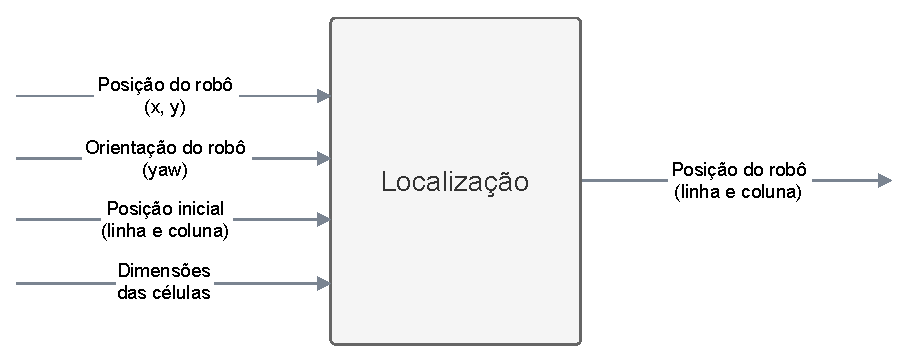
\includegraphics[width=1\textwidth]
	{Figures/especificacao_funcional_localizacao}
	\label{fig:especificacao_funcional_localizacao}
	\source{Própria Autoria}
\end{figure}

\subsection{Percepção}
\label{ssec:funcionalidade_percepcao} 
Para que o \textit{micromouse} consiga se locomover pelo labirinto, é necessário reconhecer os possíveis caminhos, identificando os obstáculos ao seu redor. Utilizando informações obtidas dos sensores infravermelho, essa funcionalidade conseguirá definir a presença de paredes nas proximidades do robô.
 
Como mencionado anteriormente, o labirinto será modelado como uma matriz $mxn$. Será utilizado um sistema de referência absoluto para o mesmo, definindo onde fica o norte, sul, leste e oeste. Com esse sistema de referência, a medida que o robô vai percorrendo o labirinto, em cada célula serão identificadas a presença de paredes. Dessa forma, essa funcionalidade irá publicar uma matriz, contendo a informação da presença de paredes ao norte, sul, leste e oeste de cada célula.

\subsubsection{Objetivo}
Identificar a presença de obstáculos ao norte, sul, leste e oeste de cada célula da matriz que representa o labirinto.

\subsubsection{Dependências}
Esse pacote depende da aquisição de dados publicados por:
\begin{itemize}
	\item Pacote de driver dos sensores infravermelho;
	\item Posição do robô, obtida do pacote de localização. 
\end{itemize}

\subsubsection{Premissas}
Para que essa funcionalidade alcance o seu propósito, assume-se que:
\begin{itemize}
	\item Os sensores infravermelho estarão conectados à Raspberry Pi e a informação dos mesmos está sendo disponibilizada corretamente;
	\item O pacote de localização estará funcionando corretamente, publicando as informações de posicionamento do robô.
\end{itemize}

\subsubsection{Saídas}
Essa funcionalidade tem como saída:
\begin{itemize}
	\item Matriz de dimensão $mxn$ com cada célula contendo valores booleanos para as seguintes variáveis:
	\begin{itemize}
		\item \textit{north}: presença de parede ao norte da célula;
		\item \textit{south}: presença de parede ao sul da célula;
		\item \textit{east}: presença de parede ao leste da célula;
		\item \textit{west}: presença de parede ao oeste da célula.
	\end{itemize}
\end{itemize}

Na Figura \ref{fig:especificacao_funcional_percepcao} pode ser visualizado quais serão as entrada e a saída da funcionalidade Percepção.

\begin{figure}[H]
	\centering
	\caption{Fluxograma ilustrativo da funcionalidade de Percepção.}
	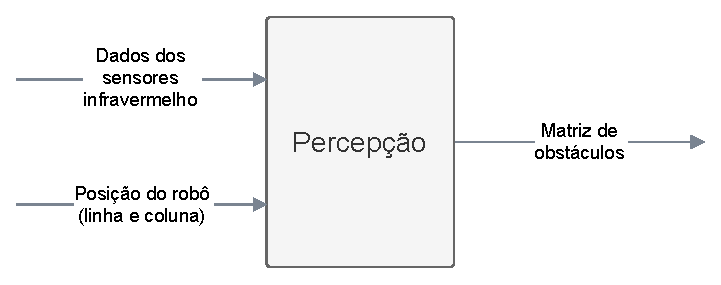
\includegraphics[width=1\textwidth]
	{Figures/especificacao_funcional_percepcao}
	\label{fig:especificacao_funcional_percepcao}
	\source{Própria Autoria}
\end{figure}

\subsection{Navegação}
\label{ssec:funcionalidade_navegacao} 
Para o robô seguir pelo melhor caminho dentro do labirinto é necessário antes que este seja conhecido por ele. Para isso, em um primeiro momento, será necessário que o micromouse percorra o labirinto somente para o seu conhecimento parcial. Então, será necessário a utilização das informações publicadas pelas funcionalidades de Percepção e Localização. Com base nelas, o sistema de navegação poderá definir os comandos necessários para que o robô execute o próximo movimento dentro do labirinto.

O micromouse será programado com 3 estratégias de solução do labirinto diferentes. Essas podem ser selecionadas pelo usuário através da interface de usuário. Primeiramente, o robô irá executar a funcionalidade de mapeamento com base no algoritmo de força bruta, que consiste em sempre que não houver obstáculos a direita, tomar este caminho, movimentando-se de modo diferente somente se for identificado impossibilidade de seguir pela direita. Após isso, o algoritmo de resolução fará com que o robô chegue ao destino final pelo percurso mais otimizado dentro das possibilidades conhecidas previamente pelo mapeamento do labirinto.

\subsubsection{Objetivo}
Planejar trajetórias a fim de garantir a correta locomoção do robô, possibilitando primeiramente o mapeamento do labirinto e após isso a chegada ao destino final pelo caminho mais rápido.

\subsubsection{Dependências}
Esse pacote depende da aquisição de dados publicados por:
\begin{itemize}
	\item Matriz de obstáculos;
	\item Posição do robô: localização do robô na matriz, no formato: [linha, coluna].
\end{itemize}

\subsubsection{Premissas}
Para que essa funcionalidade alcance o seu propósito, assume-se que:
\begin{itemize}
	\item Correto funcionamento dos pacotes de localização e percepção;
	\item Os drivers de potências dos motores estarão conectados à Raspberry Pi e o driver \gls*{ros} e o sistema de controle dos movimentos do robô estejam funcionando corretamente.
\end{itemize}

\subsubsection{Saída}
Essa funcionalidade tem como saídas:
\begin{itemize}
	\item Comandos de movimentação.
\end{itemize}

As entradas e saída da funcionalidade Navegação podem ser visualizadas na Figura \ref{fig:especificacao_funcional_navegacao}.

\begin{figure}[H]
	\centering
	\caption{Fluxograma ilustrativo da funcionalidade de Navegação.}
	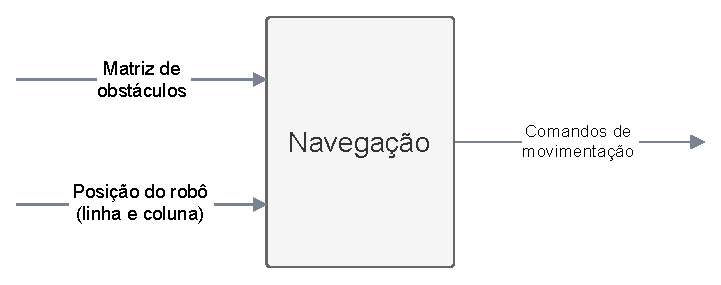
\includegraphics[width=1\textwidth]
	{Figures/especificacao_funcional_navegacao}
	\label{fig:especificacao_funcional_navegacao}
	\source{Própria Autoria}
\end{figure}

\subsection{Usabilidade}
\label{ssec:funcionalidade_usabilidade} 
Para permitir que o usuário interaja com o robô, algumas interfaces são disponibilizadas. A primeira delas consiste do acesso via \gls*{ssh} que perimite o acesso remoto do robô. Usando essa interface é possível acessar a linha de comando do robô para realizar configurações do dispositivo de processamento, compilação de códigos fonte, configuração de parâmetros do robô e execução tanto das rotinas de demonstração do robô quanto das rotinas de resolução de labirintos. Já para que o usuário exerça interação com a plataforma sem a necessidade do acesso remoto, é disponibilizado botões e um buzzer. Esses dois elementos, são utilizados principalmente em competições para facilitar o manuseio do robô.
 
Por fim, quando não utilizado em competições, o mapa do labirinto pode ser visualizado no RViz (visualizador 3D do \textit{framework} \gls*{ros}) a medida em que ele é percorrido pela plataforma móvel.

\subsubsection{Objetivo}
Permitir que o usuário acesse e edite configurações, execute comandos e monitore o estado do robô.

\subsubsection{Dependências}
Esse pacote depende da aquisição de dados publicados por:
\begin{itemize}
	\item Driver do Buzzer;
	\item Driver dos botões;
	\item Módulo de Localização;
	\item Módulo de Percepção.
\end{itemize}

\subsubsection{Premissas}
Para que essa funcionalidade alcance o seu propósito, assume-se que:
\begin{itemize}
	\item Uma rede comunicação Wireless com a plataforma esteja disponível;
	\item O acesso via SSH seja configurado previamente;
	\item O Buzzer esteja conectado a Raspberry PI e o \gls*{ros} driver esteja funcionando corretamente;
	\item  Os módulos de Percepção e Localização estejam funcionando corretamente.
\end{itemize}

\subsubsection{Saídas}
Essa funcionalidade tem como saídas:
\begin{itemize}
	\item Alertas sonoros;
	\item Mapa do labirinto (\textit{Occupancy Grid});
	\item Status do robô.
\end{itemize}

As entradas e saída da funcionalidade Navegação podem ser visualizadas na Figura \ref{fig:especificacao_funcional_usabilidade}.

\begin{figure}[H]
	\centering
	\caption{Fluxograma ilustrativo da funcionalidade de Usabilidade.}
	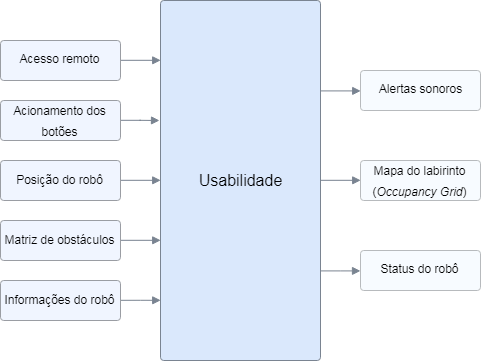
\includegraphics[width=1\textwidth]
	{Figures/especificacao_funcional_usabilidade}
	\label{fig:especificacao_funcional_usabilidade}
	\source{Própria Autoria}
\end{figure}

%--------- NEW SECTION ----------------------
\section{Simulação}
\label{sec:Simulacao}
O ambiente de simulação do robô foi realizado dentro do Gazebo \cite{Koenig2004} na versão 7.0.0, uma vez que o simulador, além de ser \textit{open source}, já possui integração nativa com o \gls*{ros} através do conjunto de pacotes providos pelo gazebo\_ros\_pkgs. Dessa forma, os mesmos recursos usado pelo \gls*{ros} para controlar o \textit{hardware} do robô, implementados através do pacote ros\_control, são também utilizados na simulação. Essa integração proporciona uma experiência mais realista do controle do robô, sendo possível inclusive a integração do ambiente de simulação com o robô real. 

A simulação será composta tanto pelo modelo do robô Doogie Mouse, quanto pelo labirinto, que serão descritos em um \gls*{urdf}, formato de arquivo padrão usado pelo \gls*{ros} para descrever o modelo de um robô, definindo-se assim os links, juntas, sensores e o funcionamento dos atuadores utilizados no Doogie Mouse, e os links e juntas usados para descrever o labirinto.

Para tanto, serão aproveitados os modelos 3D gerados na seção \ref{sec:modelo_mecanico}, para a constituição da malha de efeito visual (a que de fato é renderizada na simulação) e da malha de colisão (na qual se calcula os contatos e colisões do robô com o mundo).

De forma a otimizar a simulação, tornando-a mais leve, o modelo do robô foi simplificado, mantendo-se apenas os componentes essenciais para sua representação: a placa inferior, sensores infravermelhos e as rodas. A partir disso, através do \textit{plugin} SolidWorks to URDF Exporter, mantido pela comunidade do \gls*{ros}, gerou o modelo \gls*{urdf} do robô.

O simulador na versão utilizada suporta apenas dois formatos de arquivo para descrição de malhas: \gls*{collada} e \gls*{stl}. Através do plugin utilizado no SolidWorks a malha é exportada em \gls*{stl}, contudo neste formato não se transporta informação de cor e textura para a simulação. Para contornar esse problema, através do SolidWorks Visualize exportou-se a malha do modelo do robô em Wavefront e então, através do Blender converteu-a para \gls*{collada} para ser renderizada na simulação. A malha de colisão por sua vez foi simplificada em um dos formatos primitivos fornecidos pelo \gls*{urdf}, um paralelepípedo, de forma a conter os limites de contato do robô. Uma representação em grafos do modelo do robô pode ser vista na Figura \ref{fig:doogie_description} e na Figura \ref{fig:doogie_description_model}, o mesmo modelo através do visualizador do ROS

\begin{figure}[H]
	\centering
	\caption{Descrição Mecânica do Doogie Mouse.}
	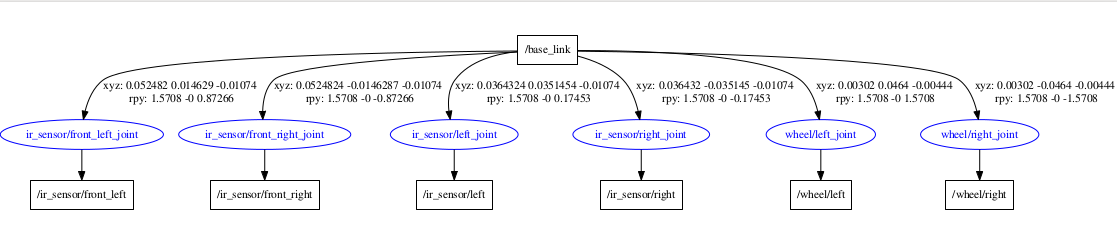
\includegraphics[width=1\textwidth]
	{Figures/doogie_description}
	\label{fig:doogie_description}
	\source{Própria Autoria}
\end{figure}

\begin{figure}[H]
	\centering
	\caption{Modelo do Doogie Mouse para Simulação.}
	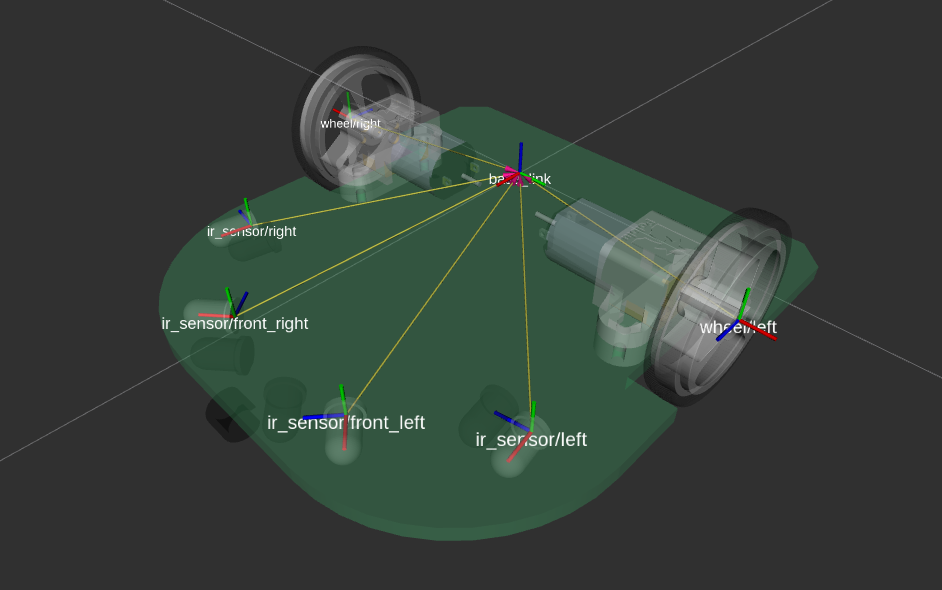
\includegraphics[width=0.5\textwidth]
	{Figures/doogie_description_model}
	\label{fig:doogie_description_model}
	\source{Própria Autoria}
\end{figure}

O labirinto, por sua vez, foi descrito como um único link cuja malha descreve tanto suas paredes quanto a base. Dentro do Gazebo, o mundo simulado já possui uma base que sustenta os objetos renderizados na simulação, sendo necessário assim somente a malha de colisão das paredes, por isso suprimiu-se a base, mantendo-a apenas como malha visual do labirinto. O mesmo procedimento utilizado para gerar o \gls*{urdf} do robô foi replicado para o labirinto, visto na Figura \ref{fig:minus_maze_description}.

\begin{figure}[H]
	\centering
	\caption{Modelo do Labirinto para Simulação.}
	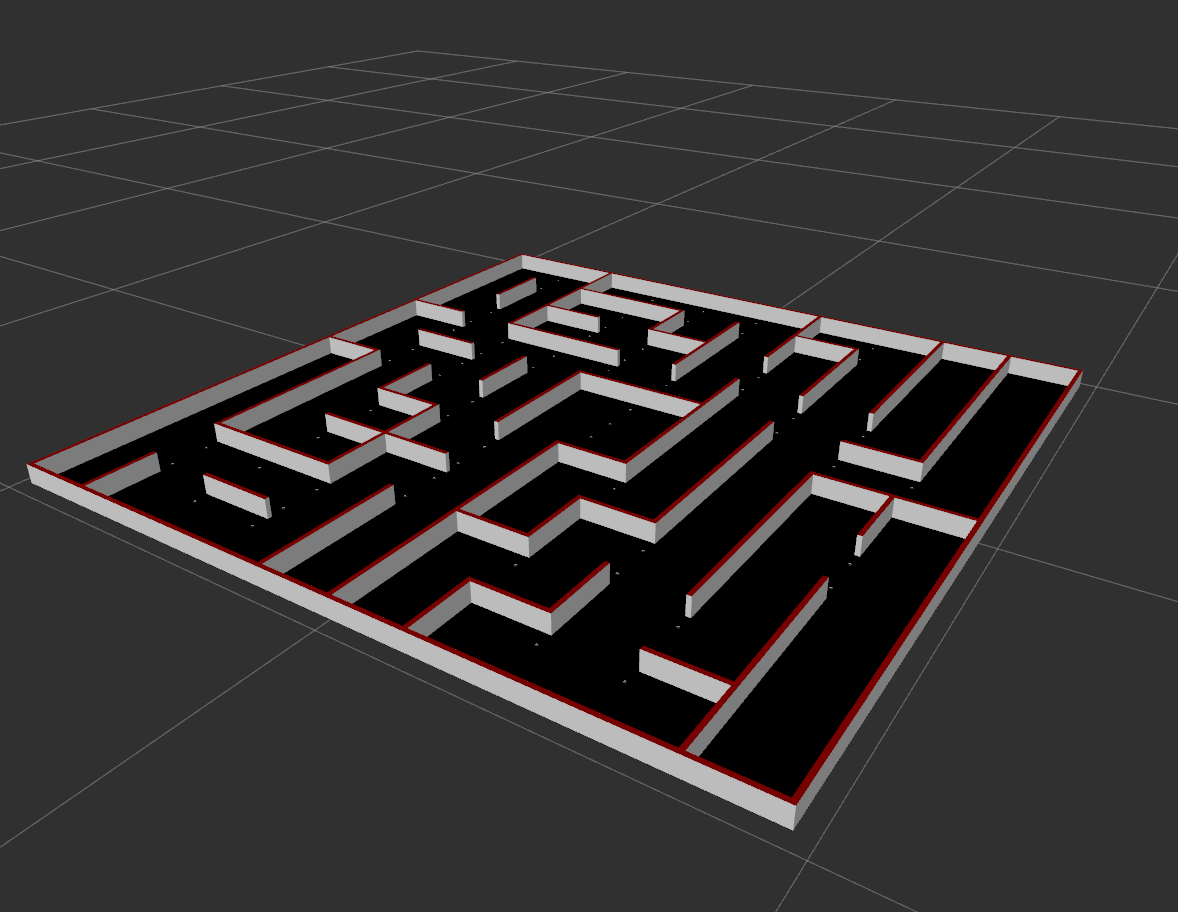
\includegraphics[width=0.5\textwidth]
	{Figures/minus_maze_description}
	\label{fig:minus_maze_description}
	\source{Própria Autoria}
\end{figure}

Também foram gerados \glspl*{urdf} utilizando as malhas em \gls*{stl} providas pelo plugin afim de realizar um ensaio para verificar como cada malha interfere na simulação e estabelecer a sua melhor configuração tomando como base os indicadores de \gls*{fps} e \gls*{rtf} fornecidos pelo Gazebo.
